Sources of systematic uncertainty are bulleted, below, with a detailed description for how each systematic is estimated.

\begin{itemize}
\item \textbf{Jet Energy Scale and Resolution - }
Uncertainties on JES and JER are estimated by shifting the corrections up and down by one standard deviation, provided by the JME POG, and taking the difference in shape between the shifted and nominal distributions as the systematic uncertainty.

\item \textbf{Muon Momentum Scale - }
Uncertainty on MES calibration with the Rochester method originates from several sources. Statistical uncertainty is estimated with the standard deviation of 100 pre-generated statistical replicas, provided in the RoccoR package~\cite{RoccoR}. Other uncertainty sources associated with corrections to the reference model MC used to derive the Rochester corrections (``Zpt,'' ``Ewk,'' ``deltaM,'' and ``Ewk2'') are availible as sets of variations in the RoccoR package. Each uncertainty is estimated by taking the difference betweeen the varied and central muon \pt. The quadrature sum of all the uncertainties (including statistical) is taken as the total. To propogate this uncertainty to final results, the analysis is repeated with muon \pt (below \SI{200}{\GeV}) shifted up and down by the total uncertainty, and the difference between the shifted and nominal distributions is taken as the systematic uncertainty on MES from Rochester corrections.

For high-\pt muons, the GE method is used to an estimate uncertainty on MES bias. A detailed study of the estimation and assignment is provided in Appendix~\ref{app:GEScaleSyst}. 


\item \textbf{Muon Momentum Resolution - }
Uncertainty on MER from Rochester corrections is factored into the MES uncertainty (detailed above). For the additional resolution smearing, an uncertainty of \SI{10}{\%} on MER is obtained by varying the binning and fit window when measuring the resolution in MC and data at the Z mass. To propogate this resolution uncertainty to final results, a muon \mom- and \pseudorap-dependent smearing is applied in the same manner as the MER corrections detailed in Section~\ref{sec:EventSelection}. Muon momenta are corrected like $\mom \rightarrow p(1 + \mathrm{Gauss}(0, \sigma(\mom,\pseudorap)0.46))$, where the 0.46 factor corresponds to a \SI{10}{\%} shift uncertainty, and $\sigma(\mom,\pseudorap)$ is the same momentum resolution parametrization as in Section~\ref{sec:EventSelection}. The analysis is then repeated with the shifted momenta, and the difference between the shifted and nominal distributions is taken as the systematic uncertainty on MER.

\item \textbf{Muon Reconstruction, Identification, Isolation, and Trigger Efficiency - }
Uncertainty on muon efficiency is estimated by shifting the muon efficiency scale factors up and down by their uncertainties, provided by the Muon POG, and taking the difference between the shifted and nominal distributions as the systematic uncertainty.


\item \textbf{B-Jet Identification Efficiency - }
Uncertainty on the b-jet identification efficiency is estimated by shifting the efficiency scale factors up and down by their uncertainty, provided the BTV POG, and taking the difference in shape between the shifted and nominal distributions as the systematic uncertainty. 

\item \textbf{Prefire Weighting - }
Uncertainty on the L1 prefire weighting in 2016 and 2017 is estimated by shifting the weights up and down by their uncertainty and taking the difference between the shifted and nominal distributions as the systematic uncertainty.

\item \textbf{Top \pt Reweighting - }
Uncertainty on the top \pt NNLO-reweighting is estimated by shifting the top \pt weight down to 1 and up the square of the nominal top \pt event weight, and taking the difference between the shifted and nominal distributions as the systematic uncertainty.  

\item \textbf{Background Normalization - }
Uncertainties in the \ZJETS, \ttbar, and diboson MC normalization factors are obtained by varying results up and down by the statistical uncertainties of the scale factors.

\item \textbf{Background Shape - }
Uncertainties in \ZJETS, \ttbar, and diboson shape are determined by varying the factorization and renormalization scale in simulation by half and twice their nominal values, which are embedded in the MC samples as weights (in total, there are eight renormalization and factorization scale variation weights, respectively: 0.5 and 0.5, 0.5 and 1.0, 0.5 and 2.0, 1.0 and 0.5, 1.0 and 2.0, 2.0 and 0.5, 2.0 and 1.0, 2.0 and 2.0). The \ZJETS, \ttbar, and diboson background normalization SFs are recomputed at preselection, within the CRs defined in Section~\ref{sec:BkgNorm}, with the scale-varied weights applied. At final selection for each leptoquark mass, event yields using the scale-varied weights (and corresponding scale-varied normalization SFs) are compared to the event yields of the central samples in the analysis by taking the percent difference. The greatest percent difference is selected as the total shape uncertainty.

\item \textbf{Luminosity - }
There are year-to-year uncorrelated, fully-correlated, and partially-correlated sources of uncertainty on the determination of the integrated luminosities~\cite{CMS:LUM-17-003}\cite{CMS:LUM-17-004}\cite{CMS:LUM-18-002} of pp collisions at \sqrtsTeV{13} in 2016, 2017, and 2018 datasets. Uncorrelated uncertainties are \SI{1.0}{\%}, \SI{2.0}{\%}, and \SI{1.5}{\%} in 2016, 2017, and 2018, respectively. Fully-correlated uncertainties are \SI{0.6}{\%}, \SI{0.9}{\%}, and \SI{2.0}{\%} in 2016, 2017, and 2018, respectively. Partially-correlated uncertainties are only correlated between 2017 and 2018, and are \SI{0.6}{\%} and \SI{0.2}{\%} in 2017 and 2018, respectively.

\item \textbf{Pile Up - }
Uncertainty on the total inelastic proton-proton cross section of \SI{69200}{\microbarn} used to model pileup is \SI{4.6}{\%}~\cite{CMS:ppInelasticCrossSection}. 
\end{itemize}

Figure~\ref{fig:totalSyst} shows the total systematic uncartainty on signal and background MC for each year as a function of leptoquark signal mass. Table~\ref{tab:SysRangesAll} lists the range of each systematic uncertainty on signal and background in each year, while Tables~\ref{tab:SysUncertainties_300}--\ref{tab:SysUncertainties_4000} show the contributions to the total uncertainty from each source of systematic in each year, for a given leptoquark mass.

\begin{figure}[H]
    \centering
    {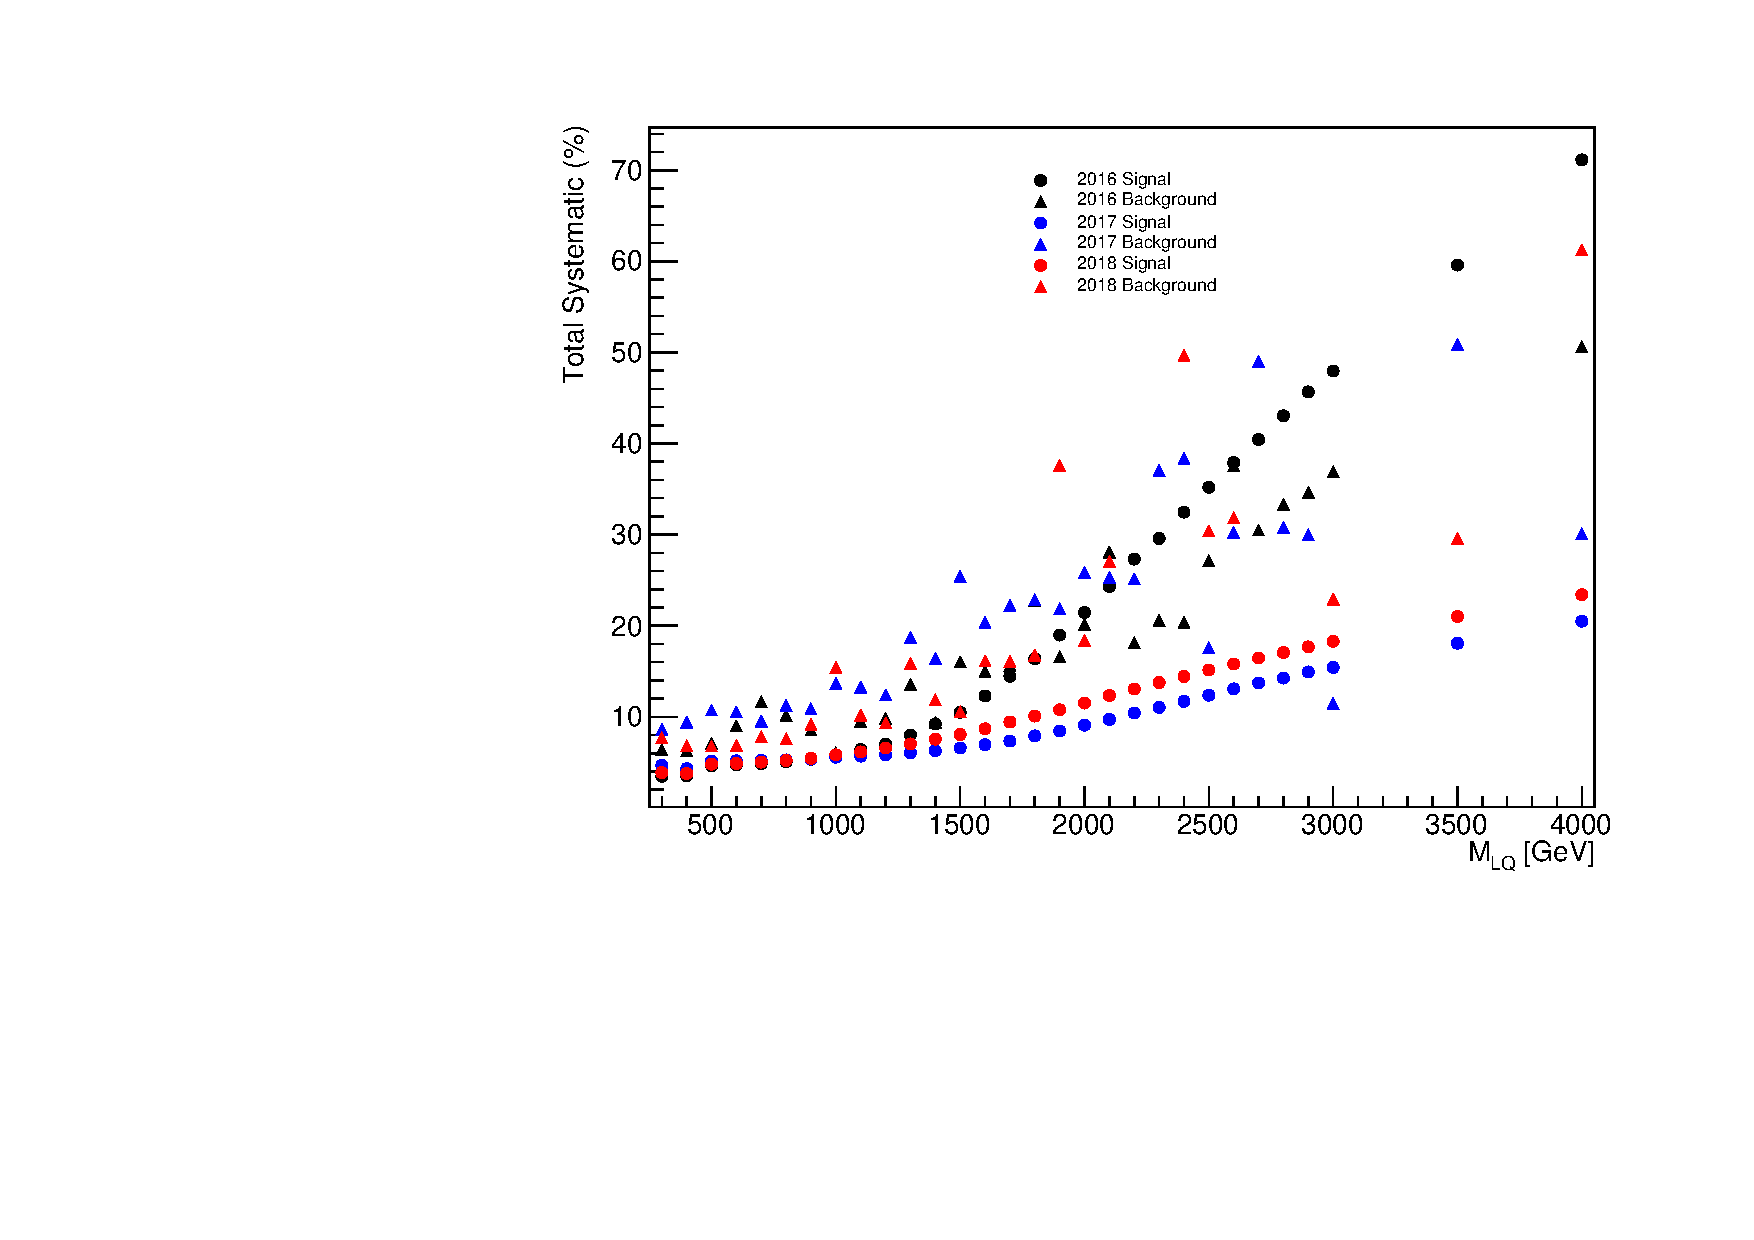
\includegraphics[width=0.8\textwidth]{Images/Analysis/TotalSysVsLQMass.pdf}}
    \caption{The total systematic uncertainty at each signal mass point in signal and background MC for 2016, 2017, and 2018.}
    \label{fig:totalSyst}
\end{figure}

\begin{table}[H]
	\begin{center}
        \begin{footnotesize}
			\caption{Range of systematic uncertainties on signal (Sig.) and background (Bkg.) in 2016, 2017, and 2018.}
			\begin{tabular}{lcccccc} \hline\hline
				 & \multicolumn{2}{c}{2016 (min--max)} & \multicolumn{2}{c}{2017 (min--max)} & \multicolumn{2}{c}{2018 (min--max)} \\
				Systematic & Sig. (\%) & Bkg. (\%) & Sig. (\%) & Bkg. (\%) & Sig. (\%) & Bkg. (\%) \\ \hline
				b-jet tagging efficiency & 0.96--7.4 & 0.3--22.79 & 1.92--6.68 & 0.39--6.97 & 0.9--14.97 & 0.37--15.31 \\
				Jet energy resolution & 0.0--0.14 & 0.25--9.39 & 0.0--0.21 & 0.31--13.2 & 0.0--0.17 & 0.17--20.66 \\
				Jet energy scale & 0.02--0.74 & 0.58--10.79 & 0.01--0.64 & 0.56--16.08 & 0.02--1.24 & 0.7--51.76 \\
				Luminosity & 1.17--1.17 & 0.14--0.44 & 2.27--2.27 & 0.27--0.91 & 2.51--2.51 & 0.33--0.65 \\
				Muon energy resolution & 0.0--0.05 & 0.08--7.64 & 0.0--0.03 & 0.09--12.62 & 0.0--0.06 & 0.15--31.86 \\
				Muon energy scale & 0.81--242.68 & 0.81--242.68 & 2.85--242.4 & 2.85--242.4 & 0.76--245.47 & 0.76--245.47 \\
				Muon identification & 1.57--1.64 & 0.07--0.55 & 0.67--0.74 & 0.11--0.38 & 0.47--0.52 & 0.07--0.16 \\
				Muon isolation & 0.31--0.31 & 0.03--0.18 & 0.23--0.24 & 0.03--0.15 & 0.16--0.17 & 0.05--0.08 \\
				Muon reconstruction & 0.55--70.62 & 0.16--33.9 & 0.38--18.78 & 0.1--3.08 & 0.31--17.37 & 0.08--2.03 \\
				Muon trigger & 0.05--0.78 & 0.02--0.52 & 0.05--0.91 & 0.02--0.83 & 0.02--0.3 & 0.03--0.08 \\
				PDF & 8.28--100.0 & 2.25--9.78 & 7.78--100.0 & 2.71--12.67 & 9.72--100.0 & 2.83--13.78 \\
				Pileup & 0.01--0.18 & 0.35--15.97 & 0.06--0.39 & 0.13--8.42 & 0.03--0.34 & 0.13--8.46 \\
				Prefire reweighting & 0.59--0.83 & 0.19--3.76 & 0.56--0.84 & 0.15--2.39 & -- & -- \\
				Top \pt reweighting & 0.0--0.0 & 0.14--1.7 & 0.0--0.0 & 0.26--2.48 & 0.0--0.0 & 0.68--2.87 \\
				TT normalization & -- & 0.07--1.31 & -- & 0.28--1.06 & -- & 0.23--0.92 \\
				TT shape & -- & 0.0--12.03 & -- & 1.73--15.59 & -- & 1.64--17.9 \\
				VV normalization & -- & 0.1--5.66 & -- & 0.19--2.34 & -- & 0.21--1.66 \\
				VV shape & -- & 0.04--6.06 & -- & 0.02--5.99 & -- & 0.09--2.98 \\
				Z normalization & -- & 0.55--15.37 & -- & 0.31--11.31 & -- & 0.33--10.16 \\
				Z shape & -- & 0.2--18.37 & -- & 0.2--4.55 & -- & 0.21--9.26 \\ \hline \hline
			\end{tabular}
			\label{tab:SysRangesAll}
        \end{footnotesize}
	\end{center}
\end{table}

%300
\begin{table}[H]
	\begin{center}
        \begin{footnotesize}
			\caption{Systematic uncertainties and their effects on signal (Sig.) and background (Bkg.) in 2016, 2017, and 2018 for $\MLQ = \SI{300}{GeV}$ final selection. All uncertainties are symmetric.}
			\begin{tabular}{lcccccc} \hline \hline
				& \multicolumn{2}{c}{2016} & \multicolumn{2}{c}{2017} & \multicolumn{2}{c}{2018} \\
				Systematic & Sig. (\%) & Bkg. (\%) & Sig. (\%) & Bkg. (\%) & Sig. (\%) & Bkg. (\%) \\ \hline
				BTAG &  0.96  &  0.3 &  1.92  &  0.42 &  0.9  &  0.38 \\
				GE &  0.02  &  0.01 &  0.02  &  0.01 &  0.02  &  0.02 \\
				JER &  0.1  &  0.3 &  0.12  &  0.57 &  0.16  &  0.44 \\
				JES &  0.74  &  0.74 &  0.64  &  0.93 &  1.24  &  1.19 \\
				LUMI16Uncorr &  1.0  &  0.11 & -- & -- & -- & -- \\
				LUMI1718 & -- & -- &  0.6  &  0.07 &  0.2  &  0.05 \\
				LUMI17Uncorr & -- & -- &  2.0  &  0.24 & -- & -- \\
				LUMI18Uncorr & -- & -- & -- & -- &  1.5  &  0.21 \\
				LUMICorr &  0.6  &  0.08 &  0.9  &  0.1 &  2.0  &  0.25 \\
				MER &  0.03  &  0.08 &  0.02  &  0.09 &  0.06  &  0.27 \\
				MES &  0.45  &  0.81 &  2.41  &  2.85 &  0.66  &  0.76 \\
				MUONHLT &  0.05  &  0.02 &  0.05  &  0.02 &  0.02  &  0.03 \\
				MUONID &  1.57  &  0.12 &  0.74  &  0.13 &  0.47  &  0.07 \\
				MUONISO &  0.31  &  0.03 &  0.24  &  0.03 &  0.17  &  0.05 \\
				MUONRECO &  0.55  &  0.16 &  0.38  &  0.1 &  0.31  &  0.08 \\
				PDF &  8.28  &  2.25 &  7.78  &  2.71 &  9.72  &  2.83 \\
				PREFIRE &  0.73  &  0.19 &  0.69  &  0.15 & -- & -- \\
				PU &  0.02  &  0.35 &  0.12  &  0.15 &  0.05  &  0.13 \\
				SHAPETT & -- &  1.58 & -- &  1.73 & -- &  1.66 \\
				SHAPEVV & -- &  0.04 & -- &  0.02 & -- &  0.09 \\
				SHAPEZ & -- &  0.25 & -- &  0.2 & -- &  0.22 \\
				TOPPT & -- &  1.38 & -- &  1.76 & -- &  1.7 \\
				TTNORM & -- &  1.31 & -- &  1.06 & -- &  0.92 \\
				VVNORM & -- &  0.2 & -- &  0.2 & -- &  0.21 \\
				ZNORM & -- &  0.55 & -- &  0.31 & -- &  0.33 \\
				Total &  8.66  &  3.63 &  8.77  &  4.94 &  10.19  &  4.15 \\ \hline \hline
			\end{tabular}
			\label{tab:SysUncertainties_300}
        \end{footnotesize}
	\end{center}
\end{table}


%400
\begin{table}[H]
	\begin{center}
        \begin{footnotesize}
			\caption{Systematic uncertainties and their effects on signal (Sig.) and background (Bkg.) in 2016, 2017, and 2018 for $\MLQ = \SI{400}{GeV}$ final selection. All uncertainties are symmetric.}
			\begin{tabular}{lcccccc} \hline \hline
				& \multicolumn{2}{c}{2016} & \multicolumn{2}{c}{2017} & \multicolumn{2}{c}{2018} \\
				Systematic & Sig. (\%) & Bkg. (\%) & Sig. (\%) & Bkg. (\%) & Sig. (\%) & Bkg. (\%) \\ \hline
				BTAG &  1.05  &  0.3 &  2.04  &  0.42 &  1.04  &  0.38 \\
				GE &  0.02  &  0.01 &  0.02  &  0.01 &  0.02  &  0.02 \\
				JER &  0.14  &  0.25 &  0.21  &  0.54 &  0.17  &  0.44 \\
				JES &  0.4  &  0.66 &  0.45  &  0.94 &  0.62  &  1.23 \\
				LUMI16Uncorr &  1.0  &  0.11 & -- & -- & -- & -- \\
				LUMI1718 & -- & -- &  0.6  &  0.07 &  0.2  &  0.05 \\
				LUMI17Uncorr & -- & -- &  2.0  &  0.24 & -- & -- \\
				LUMI18Uncorr & -- & -- & -- & -- &  1.5  &  0.21 \\
				LUMICorr &  0.6  &  0.08 &  0.9  &  0.1 &  2.0  &  0.26 \\
				MER &  0.03  &  0.09 &  0.02  &  0.1 &  0.04  &  0.27 \\
				MES &  0.25  &  0.8 &  1.27  &  2.89 &  0.36  &  0.78 \\
				MUONHLT &  0.07  &  0.02 &  0.07  &  0.02 &  0.03  &  0.03 \\
				MUONID &  1.58  &  0.12 &  0.72  &  0.13 &  0.48  &  0.07 \\
				MUONISO &  0.31  &  0.03 &  0.24  &  0.03 &  0.17  &  0.05 \\
				MUONRECO &  0.69  &  0.16 &  0.47  &  0.1 &  0.37  &  0.08 \\
				PDF &  8.28  &  2.26 &  7.78  &  2.72 &  9.72  &  2.84 \\
				PREFIRE &  0.79  &  0.2 &  0.75  &  0.15 & -- & -- \\
				PU &  0.04  &  0.36 &  0.1  &  0.15 &  0.08  &  0.13 \\
				SHAPETT & -- &  1.58 & -- &  1.73 & -- &  1.67 \\
				SHAPEVV & -- &  0.04 & -- &  0.02 & -- &  0.09 \\
				SHAPEZ & -- &  0.24 & -- &  0.2 & -- &  0.22 \\
				TOPPT & -- &  1.38 & -- &  1.77 & -- &  1.71 \\
				TTNORM & -- &  1.31 & -- &  1.06 & -- &  0.92 \\
				VVNORM & -- &  0.2 & -- &  0.2 & -- &  0.21 \\
				ZNORM & -- &  0.55 & -- &  0.31 & -- &  0.33 \\
				Total &  8.66  &  3.62 &  8.55  &  4.97 &  10.14  &  4.18 \\ \hline \hline
			\end{tabular}
			\label{tab:SysUncertainties_400}
        \end{footnotesize}
	\end{center}
\end{table}


%500
\begin{table}[H]
	\begin{center}
        \begin{footnotesize}
			\caption{Systematic uncertainties and their effects on signal (Sig.) and background (Bkg.) in 2016, 2017, and 2018 for $\MLQ = \SI{500}{GeV}$ final selection. All uncertainties are symmetric.}
			\begin{tabular}{lcccccc} \hline \hline
				& \multicolumn{2}{c}{2016} & \multicolumn{2}{c}{2017} & \multicolumn{2}{c}{2018} \\
				Systematic & Sig. (\%) & Bkg. (\%) & Sig. (\%) & Bkg. (\%) & Sig. (\%) & Bkg. (\%) \\ \hline
				BTAG &  1.2  &  0.31 &  2.15  &  0.39 &  1.28  &  0.37 \\
				GE &  0.04  &  0.03 &  0.04  &  0.02 &  0.04  &  0.04 \\
				JER &  0.06  &  0.27 &  0.13  &  0.38 &  0.06  &  0.35 \\
				JES &  0.23  &  0.71 &  0.26  &  0.73 &  0.31  &  1.04 \\
				LUMI16Uncorr &  1.0  &  0.11 & -- & -- & -- & -- \\
				LUMI1718 & -- & -- &  0.6  &  0.07 &  0.2  &  0.05 \\
				LUMI17Uncorr & -- & -- &  2.0  &  0.24 & -- & -- \\
				LUMI18Uncorr & -- & -- & -- & -- &  1.5  &  0.22 \\
				LUMICorr &  0.6  &  0.08 &  0.9  &  0.1 &  2.0  &  0.26 \\
				MER &  0.02  &  0.17 &  0.02  &  0.17 &  0.05  &  0.19 \\
				MES &  0.14  &  0.83 &  0.73  &  3.02 &  0.18  &  0.81 \\
				MUONHLT &  0.1  &  0.02 &  0.1  &  0.02 &  0.04  &  0.03 \\
				MUONID &  1.59  &  0.12 &  0.72  &  0.13 &  0.48  &  0.07 \\
				MUONISO &  0.31  &  0.03 &  0.24  &  0.03 &  0.16  &  0.05 \\
				MUONRECO &  0.89  &  0.17 &  0.58  &  0.11 &  0.45  &  0.09 \\
				PDF &  8.28  &  2.34 &  7.87  &  2.94 &  9.72  &  3.07 \\
				PREFIRE &  0.8  &  0.24 &  0.79  &  0.19 & -- & -- \\
				PU &  0.1  &  0.4 &  0.06  &  0.13 &  0.11  &  0.17 \\
				SHAPETT & -- &  1.6 & -- &  1.8 & -- &  1.72 \\
				SHAPEVV & -- &  0.04 & -- &  0.02 & -- &  0.09 \\
				SHAPEZ & -- &  0.2 & -- &  0.22 & -- &  0.23 \\
				TOPPT & -- &  1.47 & -- &  1.91 & -- &  1.84 \\
				TTNORM & -- &  1.3 & -- &  1.05 & -- &  0.91 \\
				VVNORM & -- &  0.21 & -- &  0.21 & -- &  0.22 \\
				ZNORM & -- &  0.56 & -- &  0.34 & -- &  0.37 \\
				Total &  8.69  &  3.74 &  8.6  &  5.19 &  10.15  &  4.36 \\ \hline \hline
			\end{tabular}
			\label{tab:SysUncertainties_500}
        \end{footnotesize}
	\end{center}
\end{table}


%600
\begin{table}[H]
	\begin{center}
        \begin{footnotesize}
			\caption{Systematic uncertainties and their effects on signal (Sig.) and background (Bkg.) in 2016, 2017, and 2018 for $\MLQ = \SI{600}{GeV}$ final selection. All uncertainties are symmetric.}
			\begin{tabular}{lcccccc} \hline \hline
				& \multicolumn{2}{c}{2016} & \multicolumn{2}{c}{2017} & \multicolumn{2}{c}{2018} \\
				Systematic & Sig. (\%) & Bkg. (\%) & Sig. (\%) & Bkg. (\%) & Sig. (\%) & Bkg. (\%) \\ \hline
				BTAG &  1.35  &  0.3 &  2.25  &  0.44 &  1.57  &  0.37 \\
				GE &  0.04  &  0.06 &  0.04  &  0.05 &  0.04  &  0.07 \\
				JER &  0.03  &  0.47 &  0.07  &  0.4 &  0.06  &  0.17 \\
				JES &  0.14  &  0.68 &  0.16  &  0.67 &  0.25  &  0.83 \\
				LUMI16Uncorr &  1.0  &  0.12 & -- & -- & -- & -- \\
				LUMI1718 & -- & -- &  0.6  &  0.08 &  0.2  &  0.05 \\
				LUMI17Uncorr & -- & -- &  2.0  &  0.26 & -- & -- \\
				LUMI18Uncorr & -- & -- & -- & -- &  1.5  &  0.23 \\
				LUMICorr &  0.6  &  0.08 &  0.9  &  0.11 &  2.0  &  0.28 \\
				MER &  0.01  &  0.11 &  0.02  &  0.25 &  0.02  &  0.15 \\
				MES &  0.09  &  0.95 &  0.43  &  3.09 &  0.12  &  0.72 \\
				MUONHLT &  0.14  &  0.02 &  0.13  &  0.02 &  0.06  &  0.03 \\
				MUONID &  1.59  &  0.13 &  0.71  &  0.12 &  0.49  &  0.08 \\
				MUONISO &  0.31  &  0.03 &  0.24  &  0.04 &  0.16  &  0.05 \\
				MUONRECO &  1.15  &  0.2 &  0.69  &  0.13 &  0.55  &  0.1 \\
				PDF &  8.28  &  2.53 &  7.87  &  3.42 &  9.72  &  3.57 \\
				PREFIRE &  0.83  &  0.33 &  0.8  &  0.29 & -- & -- \\
				PU &  0.18  &  0.53 &  0.16  &  0.18 &  0.08  &  0.26 \\
				SHAPETT & -- &  2.57 & -- &  1.81 & -- &  1.64 \\
				SHAPEVV & -- &  0.04 & -- &  0.04 & -- &  0.1 \\
				SHAPEZ & -- &  0.35 & -- &  0.32 & -- &  0.21 \\
				TOPPT & -- &  1.57 & -- &  2.09 & -- &  2.01 \\
				TTNORM & -- &  1.27 & -- &  1.03 & -- &  0.89 \\
				VVNORM & -- &  0.24 & -- &  0.24 & -- &  0.24 \\
				ZNORM & -- &  0.68 & -- &  0.41 & -- &  0.45 \\
				Total &  8.74  &  4.46 &  8.61  &  5.6 &  10.19  &  4.71 \\ \hline \hline
			\end{tabular}
			\label{tab:SysUncertainties_600}
        \end{footnotesize}
	\end{center}
\end{table}


%700
\begin{table}[H]
	\begin{center}
        \begin{footnotesize}
			\caption{Systematic uncertainties and their effects on signal (Sig.) and background (Bkg.) in 2016, 2017, and 2018 for $\MLQ = \SI{700}{GeV}$ final selection. All uncertainties are symmetric.}
			\begin{tabular}{lcccccc} \hline \hline
				& \multicolumn{2}{c}{2016} & \multicolumn{2}{c}{2017} & \multicolumn{2}{c}{2018} \\
				Systematic & Sig. (\%) & Bkg. (\%) & Sig. (\%) & Bkg. (\%) & Sig. (\%) & Bkg. (\%) \\ \hline
				BTAG &  1.53  &  0.49 &  2.34  &  0.66 &  1.91  &  0.51 \\
				GE &  0.05  &  0.08 &  0.05  &  0.07 &  0.05  &  0.09 \\
				JER &  0.01  &  0.51 &  0.05  &  0.31 &  0.03  &  0.28 \\
				JES &  0.1  &  0.58 &  0.12  &  0.56 &  0.17  &  0.7 \\
				LUMI16Uncorr &  1.0  &  0.13 & -- & -- & -- & -- \\
				LUMI1718 & -- & -- &  0.6  &  0.08 &  0.2  &  0.05 \\
				LUMI17Uncorr & -- & -- &  2.0  &  0.28 & -- & -- \\
				LUMI18Uncorr & -- & -- & -- & -- &  1.5  &  0.24 \\
				LUMICorr &  0.6  &  0.09 &  0.9  &  0.12 &  2.0  &  0.3 \\
				MER &  0.05  &  0.24 &  0.01  &  0.22 &  0.01  &  0.19 \\
				MES &  0.06  &  1.27 &  0.27  &  3.01 &  0.07  &  0.73 \\
				MUONHLT &  0.19  &  0.02 &  0.18  &  0.02 &  0.08  &  0.03 \\
				MUONID &  1.59  &  0.15 &  0.7  &  0.12 &  0.49  &  0.09 \\
				MUONISO &  0.31  &  0.04 &  0.24  &  0.04 &  0.16  &  0.05 \\
				MUONRECO &  1.44  &  0.24 &  0.81  &  0.15 &  0.66  &  0.12 \\
				PDF &  8.28  &  2.83 &  7.87  &  4.11 &  9.72  &  4.2 \\
				PREFIRE &  0.82  &  0.46 &  0.81  &  0.42 & -- & -- \\
				PU &  0.02  &  0.58 &  0.14  &  0.2 &  0.06  &  0.19 \\
				SHAPETT & -- &  3.55 & -- &  1.93 & -- &  1.84 \\
				SHAPEVV & -- &  0.05 & -- &  0.04 & -- &  0.12 \\
				SHAPEZ & -- &  0.43 & -- &  0.32 & -- &  0.27 \\
				TOPPT & -- &  1.64 & -- &  2.22 & -- &  2.14 \\
				TTNORM & -- &  1.25 & -- &  1.01 & -- &  0.87 \\
				VVNORM & -- &  0.29 & -- &  0.27 & -- &  0.29 \\
				ZNORM & -- &  0.72 & -- &  0.51 & -- &  0.54 \\
				Total &  8.81  &  5.37 &  8.64  &  6.11 &  10.26  &  5.33 \\ \hline \hline
			\end{tabular}
			\label{tab:SysUncertainties_700}
        \end{footnotesize}
	\end{center}
\end{table}


%800
\begin{table}[H]
	\begin{center}
        \begin{footnotesize}
			\caption{Systematic uncertainties and their effects on signal (Sig.) and background (Bkg.) in 2016, 2017, and 2018 for $\MLQ = \SI{800}{GeV}$ final selection. All uncertainties are symmetric.}
			\begin{tabular}{lcccccc} \hline \hline
				& \multicolumn{2}{c}{2016} & \multicolumn{2}{c}{2017} & \multicolumn{2}{c}{2018} \\
				Systematic & Sig. (\%) & Bkg. (\%) & Sig. (\%) & Bkg. (\%) & Sig. (\%) & Bkg. (\%) \\ \hline
				BTAG &  1.69  &  0.62 &  2.42  &  0.92 &  2.31  &  0.74 \\
				GE &  0.07  &  0.16 &  0.07  &  0.15 &  0.07  &  0.17 \\
				JER &  0.01  &  1.57 &  0.05  &  0.46 &  0.01  &  0.26 \\
				JES &  0.06  &  0.74 &  0.09  &  0.85 &  0.13  &  0.78 \\
				LUMI16Uncorr &  1.0  &  0.15 & -- & -- & -- & -- \\
				LUMI1718 & -- & -- &  0.6  &  0.09 &  0.2  &  0.06 \\
				LUMI17Uncorr & -- & -- &  2.0  &  0.3 & -- & -- \\
				LUMI18Uncorr & -- & -- & -- & -- &  1.5  &  0.26 \\
				LUMICorr &  0.6  &  0.1 &  0.9  &  0.13 &  2.0  &  0.32 \\
				MER &  0.0  &  0.27 &  0.02  &  0.55 &  0.02  &  0.4 \\
				MES &  0.04  &  0.75 &  0.16  &  3.03 &  0.06  &  0.8 \\
				MUONHLT &  0.24  &  0.03 &  0.22  &  0.02 &  0.1  &  0.03 \\
				MUONID &  1.6  &  0.17 &  0.7  &  0.11 &  0.5  &  0.1 \\
				MUONISO &  0.31  &  0.04 &  0.24  &  0.05 &  0.16  &  0.06 \\
				MUONRECO &  1.86  &  0.29 &  0.94  &  0.18 &  0.81  &  0.14 \\
				PDF &  8.28  &  3.17 &  7.87  &  4.75 &  10.59  &  4.82 \\
				PREFIRE &  0.83  &  0.63 &  0.83  &  0.56 & -- & -- \\
				PU &  0.11  &  0.52 &  0.14  &  0.35 &  0.04  &  0.31 \\
				SHAPETT & -- &  4.59 & -- &  3.27 & -- &  3.16 \\
				SHAPEVV & -- &  0.04 & -- &  0.04 & -- &  0.19 \\
				SHAPEZ & -- &  0.39 & -- &  0.37 & -- &  0.31 \\
				TOPPT & -- &  1.64 & -- &  2.3 & -- &  2.19 \\
				TTNORM & -- &  1.21 & -- &  0.98 & -- &  0.84 \\
				VVNORM & -- &  0.32 & -- &  0.31 & -- &  0.36 \\
				ZNORM & -- &  0.76 & -- &  0.65 & -- &  0.64 \\
				Total &  8.93  &  6.4 &  8.67  &  7.21 &  11.17  &  6.46 \\ \hline \hline
			\end{tabular}
			\label{tab:SysUncertainties_800}
        \end{footnotesize}
	\end{center}
\end{table}


%900
\begin{table}[H]
	\begin{center}
        \begin{footnotesize}
			\caption{Systematic uncertainties and their effects on signal (Sig.) and background (Bkg.) in 2016, 2017, and 2018 for $\MLQ = \SI{900}{GeV}$ final selection. All uncertainties are symmetric.}
			\begin{tabular}{lcccccc} \hline \hline
				& \multicolumn{2}{c}{2016} & \multicolumn{2}{c}{2017} & \multicolumn{2}{c}{2018} \\
				Systematic & Sig. (\%) & Bkg. (\%) & Sig. (\%) & Bkg. (\%) & Sig. (\%) & Bkg. (\%) \\ \hline
				BTAG &  1.86  &  0.78 &  2.53  &  1.19 &  2.73  &  0.99 \\
				GE &  0.12  &  0.18 &  0.12  &  0.16 &  0.12  &  0.18 \\
				JER &  0.01  &  0.54 &  0.02  &  0.72 &  0.06  &  0.78 \\
				JES &  0.07  &  0.77 &  0.09  &  0.89 &  0.12  &  1.32 \\
				LUMI16Uncorr &  1.0  &  0.16 & -- & -- & -- & -- \\
				LUMI1718 & -- & -- &  0.6  &  0.1 &  0.2  &  0.06 \\
				LUMI17Uncorr & -- & -- &  2.0  &  0.33 & -- & -- \\
				LUMI18Uncorr & -- & -- & -- & -- &  1.5  &  0.27 \\
				LUMICorr &  0.6  &  0.11 &  0.9  &  0.14 &  2.0  &  0.34 \\
				MER &  0.01  &  0.34 &  0.01  &  0.36 &  0.02  &  0.66 \\
				MES &  0.02  &  0.8 &  0.11  &  3.27 &  0.02  &  1.1 \\
				MUONHLT &  0.29  &  0.03 &  0.27  &  0.03 &  0.12  &  0.03 \\
				MUONID &  1.6  &  0.2 &  0.69  &  0.11 &  0.5  &  0.11 \\
				MUONISO &  0.31  &  0.05 &  0.23  &  0.05 &  0.16  &  0.06 \\
				MUONRECO &  2.4  &  0.34 &  1.12  &  0.21 &  1.0  &  0.16 \\
				PDF &  8.28  &  3.57 &  7.87  &  5.44 &  11.96  &  5.4 \\
				PREFIRE &  0.8  &  0.79 &  0.84  &  0.71 & -- & -- \\
				PU &  0.06  &  0.5 &  0.16  &  0.43 &  0.04  &  0.3 \\
				SHAPETT & -- &  5.77 & -- &  4.99 & -- &  4.6 \\
				SHAPEVV & -- &  0.05 & -- &  0.06 & -- &  0.21 \\
				SHAPEZ & -- &  0.33 & -- &  0.25 & -- &  0.42 \\
				TOPPT & -- &  1.65 & -- &  2.34 & -- &  2.2 \\
				TTNORM & -- &  1.19 & -- &  0.95 & -- &  0.82 \\
				VVNORM & -- &  0.37 & -- &  0.36 & -- &  0.41 \\
				ZNORM & -- &  0.72 & -- &  0.74 & -- &  0.82 \\
				Total &  9.09  &  7.37 &  8.73  &  8.72 &  12.57  &  7.89 \\ \hline \hline
			\end{tabular}
			\label{tab:SysUncertainties_900}
        \end{footnotesize}
	\end{center}
\end{table}


%1000
\begin{table}[H]
	\begin{center}
        \begin{footnotesize}
			\caption{Systematic uncertainties and their effects on signal (Sig.) and background (Bkg.) in 2016, 2017, and 2018 for $\MLQ = \SI{1000}{GeV}$ final selection. All uncertainties are symmetric.}
			\begin{tabular}{lcccccc} \hline \hline
				& \multicolumn{2}{c}{2016} & \multicolumn{2}{c}{2017} & \multicolumn{2}{c}{2018} \\
				Systematic & Sig. (\%) & Bkg. (\%) & Sig. (\%) & Bkg. (\%) & Sig. (\%) & Bkg. (\%) \\ \hline
				BTAG &  2.07  &  1.0 &  2.63  &  1.49 &  3.2  &  1.26 \\
				GE &  0.23  &  0.28 &  0.23  &  0.26 &  0.23  &  0.28 \\
				JER &  0.01  &  0.44 &  0.02  &  0.58 &  0.01  &  1.39 \\
				JES &  0.06  &  1.13 &  0.06  &  0.92 &  0.11  &  1.81 \\
				LUMI16Uncorr &  1.0  &  0.18 & -- & -- & -- & -- \\
				LUMI1718 & -- & -- &  0.6  &  0.11 &  0.2  &  0.06 \\
				LUMI17Uncorr & -- & -- &  2.0  &  0.36 & -- & -- \\
				LUMI18Uncorr & -- & -- & -- & -- &  1.5  &  0.28 \\
				LUMICorr &  0.6  &  0.12 &  0.9  &  0.16 &  2.0  &  0.35 \\
				MER &  0.02  &  0.5 &  0.0  &  0.23 &  0.02  &  0.46 \\
				MES &  0.01  &  1.18 &  0.08  &  3.61 &  0.05  &  1.04 \\
				MUONHLT &  0.33  &  0.03 &  0.33  &  0.03 &  0.14  &  0.03 \\
				MUONID &  1.61  &  0.23 &  0.69  &  0.12 &  0.5  &  0.11 \\
				MUONISO &  0.31  &  0.06 &  0.23  &  0.06 &  0.16  &  0.06 \\
				MUONRECO &  3.01  &  0.39 &  1.35  &  0.25 &  1.23  &  0.19 \\
				PDF &  9.43  &  3.95 &  9.26  &  6.13 &  13.41  &  6.03 \\
				PREFIRE &  0.82  &  0.94 &  0.82  &  0.83 & -- & -- \\
				PU &  0.09  &  0.8 &  0.22  &  0.5 &  0.03  &  0.34 \\
				SHAPETT & -- &  6.87 & -- &  6.35 & -- &  6.38 \\
				SHAPEVV & -- &  0.09 & -- &  0.08 & -- &  0.26 \\
				SHAPEZ & -- &  0.41 & -- &  0.33 & -- &  0.39 \\
				TOPPT & -- &  1.62 & -- &  2.35 & -- &  2.25 \\
				TTNORM & -- &  1.15 & -- &  0.91 & -- &  0.79 \\
				VVNORM & -- &  0.43 & -- &  0.42 & -- &  0.43 \\
				ZNORM & -- &  0.82 & -- &  0.85 & -- &  1.03 \\
				Total &  10.35  &  8.59 &  10.05  &  10.15 &  14.08  &  9.63 \\ \hline \hline
			\end{tabular}
			\label{tab:SysUncertainties_1000}
        \end{footnotesize}
	\end{center}
\end{table}


%1100
\begin{table}[H]
	\begin{center}
        \begin{footnotesize}
			\caption{Systematic uncertainties and their effects on signal (Sig.) and background (Bkg.) in 2016, 2017, and 2018 for $\MLQ = \SI{1100}{GeV}$ final selection. All uncertainties are symmetric.}
			\begin{tabular}{lcccccc} \hline \hline
				& \multicolumn{2}{c}{2016} & \multicolumn{2}{c}{2017} & \multicolumn{2}{c}{2018} \\
				Systematic & Sig. (\%) & Bkg. (\%) & Sig. (\%) & Bkg. (\%) & Sig. (\%) & Bkg. (\%) \\ \hline
				BTAG &  2.28  &  1.37 &  2.76  &  1.77 &  3.63  &  1.58 \\
				GE &  0.28  &  0.46 &  0.28  &  0.44 &  0.28  &  0.46 \\
				JER &  0.01  &  0.82 &  0.01  &  0.9 &  0.02  &  0.63 \\
				JES &  0.05  &  1.66 &  0.05  &  0.93 &  0.11  &  1.88 \\
				LUMI16Uncorr &  1.0  &  0.2 & -- & -- & -- & -- \\
				LUMI1718 & -- & -- &  0.6  &  0.12 &  0.2  &  0.06 \\
				LUMI17Uncorr & -- & -- &  2.0  &  0.38 & -- & -- \\
				LUMI18Uncorr & -- & -- & -- & -- &  1.5  &  0.28 \\
				LUMICorr &  0.6  &  0.13 &  0.9  &  0.17 &  2.0  &  0.35 \\
				MER &  0.04  &  0.97 &  0.0  &  0.41 &  0.01  &  0.54 \\
				MES &  0.01  &  1.4 &  0.04  &  3.29 &  0.02  &  1.21 \\
				MUONHLT &  0.39  &  0.04 &  0.38  &  0.04 &  0.16  &  0.04 \\
				MUONID &  1.61  &  0.27 &  0.69  &  0.15 &  0.5  &  0.11 \\
				MUONISO &  0.31  &  0.07 &  0.23  &  0.06 &  0.16  &  0.06 \\
				MUONRECO &  3.9  &  0.46 &  1.58  &  0.28 &  1.54  &  0.21 \\
				PDF &  9.51  &  4.44 &  10.06  &  6.72 &  15.17  &  6.59 \\
				PREFIRE &  0.79  &  1.13 &  0.81  &  0.95 & -- & -- \\
				PU &  0.06  &  1.17 &  0.14  &  0.71 &  0.12  &  0.37 \\
				SHAPETT & -- &  8.15 & -- &  7.58 & -- &  7.46 \\
				SHAPEVV & -- &  0.15 & -- &  0.11 & -- &  0.28 \\
				SHAPEZ & -- &  0.8 & -- &  0.46 & -- &  0.53 \\
				TOPPT & -- &  1.62 & -- &  2.37 & -- &  2.27 \\
				TTNORM & -- &  1.13 & -- &  0.88 & -- &  0.77 \\
				VVNORM & -- &  0.49 & -- &  0.51 & -- &  0.47 \\
				ZNORM & -- &  0.62 & -- &  1.02 & -- &  1.32 \\
				Total &  10.76  &  10.14 &  10.86  &  11.32 &  15.89  &  10.77 \\ \hline \hline
			\end{tabular}
			\label{tab:SysUncertainties_1100}
        \end{footnotesize}
	\end{center}
\end{table}


%1200
\begin{table}[H]
	\begin{center}
        \begin{footnotesize}
			\caption{Systematic uncertainties and their effects on signal (Sig.) and background (Bkg.) in 2016, 2017, and 2018 for $\MLQ = \SI{1200}{GeV}$ final selection. All uncertainties are symmetric.}
			\begin{tabular}{lcccccc} \hline \hline
				& \multicolumn{2}{c}{2016} & \multicolumn{2}{c}{2017} & \multicolumn{2}{c}{2018} \\
				Systematic & Sig. (\%) & Bkg. (\%) & Sig. (\%) & Bkg. (\%) & Sig. (\%) & Bkg. (\%) \\ \hline
				BTAG &  2.49  &  1.56 &  2.87  &  2.03 &  4.19  &  1.8 \\
				GE &  0.41  &  0.61 &  0.41  &  0.59 &  0.41  &  0.61 \\
				JER &  0.0  &  1.7 &  0.01  &  1.27 &  0.0  &  0.73 \\
				JES &  0.05  &  2.86 &  0.06  &  1.97 &  0.08  &  2.06 \\
				LUMI16Uncorr &  1.0  &  0.21 & -- & -- & -- & -- \\
				LUMI1718 & -- & -- &  0.6  &  0.13 &  0.2  &  0.06 \\
				LUMI17Uncorr & -- & -- &  2.0  &  0.42 & -- & -- \\
				LUMI18Uncorr & -- & -- & -- & -- &  1.5  &  0.3 \\
				LUMICorr &  0.6  &  0.14 &  0.9  &  0.19 &  2.0  &  0.37 \\
				MER &  0.01  &  0.76 &  0.01  &  0.86 &  0.01  &  0.94 \\
				MES &  0.01  &  1.11 &  0.04  &  3.3 &  0.01  &  1.09 \\
				MUONHLT &  0.42  &  0.04 &  0.43  &  0.04 &  0.18  &  0.04 \\
				MUONID &  1.61  &  0.28 &  0.69  &  0.18 &  0.5  &  0.12 \\
				MUONISO &  0.31  &  0.07 &  0.23  &  0.07 &  0.16  &  0.07 \\
				MUONRECO &  4.75  &  0.54 &  1.86  &  0.32 &  1.84  &  0.24 \\
				PDF &  10.19  &  4.77 &  10.06  &  7.32 &  17.69  &  7.14 \\
				PREFIRE &  0.78  &  1.19 &  0.81  &  1.05 & -- & -- \\
				PU &  0.08  &  1.11 &  0.23  &  1.04 &  0.24  &  0.69 \\
				SHAPETT & -- &  9.2 & -- &  8.76 & -- &  8.48 \\
				SHAPEVV & -- &  0.17 & -- &  0.17 & -- &  0.23 \\
				SHAPEZ & -- &  0.61 & -- &  0.63 & -- &  0.54 \\
				TOPPT & -- &  1.57 & -- &  2.37 & -- &  2.27 \\
				TTNORM & -- &  1.05 & -- &  0.84 & -- &  0.75 \\
				VVNORM & -- &  0.54 & -- &  0.62 & -- &  0.43 \\
				ZNORM & -- &  1.28 & -- &  1.07 & -- &  1.49 \\
				Total &  11.73  &  11.49 &  10.94  &  12.76 &  18.46  &  11.94 \\ \hline \hline
			\end{tabular}
			\label{tab:SysUncertainties_1200}
        \end{footnotesize}
	\end{center}
\end{table}


%1300
\begin{table}[H]
	\begin{center}
        \begin{footnotesize}
			\caption{Systematic uncertainties and their effects on signal (Sig.) and background (Bkg.) in 2016, 2017, and 2018 for $\MLQ = \SI{1300}{GeV}$ final selection. All uncertainties are symmetric.}
			\begin{tabular}{lcccccc} \hline \hline
				& \multicolumn{2}{c}{2016} & \multicolumn{2}{c}{2017} & \multicolumn{2}{c}{2018} \\
				Systematic & Sig. (\%) & Bkg. (\%) & Sig. (\%) & Bkg. (\%) & Sig. (\%) & Bkg. (\%) \\ \hline
				BTAG &  2.72  &  1.88 &  3.05  &  2.44 &  4.71  &  2.12 \\
				GE &  0.53  &  0.77 &  0.53  &  0.75 &  0.53  &  0.77 \\
				JER &  0.0  &  0.63 &  0.02  &  2.3 &  0.01  &  0.9 \\
				JES &  0.04  &  2.23 &  0.05  &  3.16 &  0.07  &  2.25 \\
				LUMI16Uncorr &  1.0  &  0.22 & -- & -- & -- & -- \\
				LUMI1718 & -- & -- &  0.6  &  0.13 &  0.2  &  0.06 \\
				LUMI17Uncorr & -- & -- &  2.0  &  0.45 & -- & -- \\
				LUMI18Uncorr & -- & -- & -- & -- &  1.5  &  0.31 \\
				LUMICorr &  0.6  &  0.14 &  0.9  &  0.2 &  2.0  &  0.39 \\
				MER &  0.01  &  0.7 &  0.03  &  0.79 &  0.02  &  1.5 \\
				MES &  0.01  &  1.28 &  0.04  &  3.93 &  0.02  &  2.76 \\
				MUONHLT &  0.47  &  0.04 &  0.47  &  0.05 &  0.19  &  0.04 \\
				MUONID &  1.62  &  0.27 &  0.69  &  0.21 &  0.5  &  0.11 \\
				MUONISO &  0.31  &  0.07 &  0.23  &  0.08 &  0.16  &  0.07 \\
				MUONRECO &  6.02  &  0.63 &  2.2  &  0.36 &  2.23  &  0.26 \\
				PDF &  13.61  &  5.01 &  10.06  &  7.84 &  21.05  &  7.73 \\
				PREFIRE &  0.77  &  1.26 &  0.8  &  1.22 & -- & -- \\
				PU &  0.14  &  1.72 &  0.18  &  1.28 &  0.12  &  0.67 \\
				SHAPETT & -- &  9.69 & -- &  9.43 & -- &  9.65 \\
				SHAPEVV & -- &  0.17 & -- &  0.25 & -- &  0.21 \\
				SHAPEZ & -- &  0.74 & -- &  0.98 & -- &  0.75 \\
				TOPPT & -- &  1.56 & -- &  2.35 & -- &  2.36 \\
				TTNORM & -- &  1.02 & -- &  0.81 & -- &  0.74 \\
				VVNORM & -- &  0.57 & -- &  0.77 & -- &  0.43 \\
				ZNORM & -- &  1.46 & -- &  1.09 & -- &  1.48 \\
				Total &  15.3  &  11.93 &  11.06  &  14.17 &  21.84  &  13.55 \\ \hline \hline
			\end{tabular}
			\label{tab:SysUncertainties_1300}
        \end{footnotesize}
	\end{center}
\end{table}


%1400
\begin{table}[H]
	\begin{center}
        \begin{footnotesize}
			\caption{Systematic uncertainties and their effects on signal (Sig.) and background (Bkg.) in 2016, 2017, and 2018 for $\MLQ = \SI{1400}{GeV}$ final selection. All uncertainties are symmetric.}
			\begin{tabular}{lcccccc} \hline \hline
				& \multicolumn{2}{c}{2016} & \multicolumn{2}{c}{2017} & \multicolumn{2}{c}{2018} \\
				Systematic & Sig. (\%) & Bkg. (\%) & Sig. (\%) & Bkg. (\%) & Sig. (\%) & Bkg. (\%) \\ \hline
				BTAG &  2.94  &  2.25 &  3.2  &  2.61 &  5.27  &  2.59 \\
				GE &  0.69  &  1.26 &  0.69  &  1.25 &  0.69  &  1.26 \\
				JER &  0.01  &  1.48 &  0.01  &  1.29 &  0.01  &  1.16 \\
				JES &  0.04  &  2.57 &  0.03  &  1.49 &  0.06  &  2.62 \\
				LUMI16Uncorr &  1.0  &  0.24 & -- & -- & -- & -- \\
				LUMI1718 & -- & -- &  0.6  &  0.14 &  0.2  &  0.06 \\
				LUMI17Uncorr & -- & -- &  2.0  &  0.48 & -- & -- \\
				LUMI18Uncorr & -- & -- & -- & -- &  1.5  &  0.32 \\
				LUMICorr &  0.6  &  0.15 &  0.9  &  0.22 &  2.0  &  0.4 \\
				MER &  0.0  &  1.14 &  0.01  &  0.93 &  0.01  &  1.3 \\
				MES &  0.0  &  1.18 &  0.01  &  3.15 &  0.01  &  1.79 \\
				MUONHLT &  0.5  &  0.05 &  0.52  &  0.06 &  0.21  &  0.04 \\
				MUONID &  1.62  &  0.32 &  0.68  &  0.23 &  0.51  &  0.11 \\
				MUONISO &  0.31  &  0.08 &  0.23  &  0.08 &  0.16  &  0.07 \\
				MUONRECO &  7.46  &  0.73 &  2.63  &  0.41 &  2.63  &  0.3 \\
				PDF &  15.84  &  5.55 &  16.42  &  8.47 &  25.09  &  8.33 \\
				PREFIRE &  0.75  &  1.41 &  0.8  &  1.34 & -- & -- \\
				PU &  0.04  &  2.05 &  0.18  &  1.3 &  0.11  &  1.08 \\
				SHAPETT & -- &  9.4 & -- &  9.6 & -- &  10.44 \\
				SHAPEVV & -- &  0.21 & -- &  0.35 & -- &  0.22 \\
				SHAPEZ & -- &  0.89 & -- &  1.1 & -- &  0.9 \\
				TOPPT & -- &  1.53 & -- &  2.33 & -- &  2.36 \\
				TTNORM & -- &  0.94 & -- &  0.76 & -- &  0.7 \\
				VVNORM & -- &  0.61 & -- &  0.8 & -- &  0.46 \\
				ZNORM & -- &  1.83 & -- &  1.42 & -- &  1.82 \\
				Total &  17.9  &  12.33 &  17.14  &  14.18 &  25.91  &  14.55 \\ \hline \hline
			\end{tabular}
			\label{tab:SysUncertainties_1400}
        \end{footnotesize}
	\end{center}
\end{table}


%1500
\begin{table}[H]
	\begin{center}
        \begin{footnotesize}
			\caption{Systematic uncertainties and their effects on signal (Sig.) and background (Bkg.) in 2016, 2017, and 2018 for $\MLQ = \SI{1500}{GeV}$ final selection. All uncertainties are symmetric.}
			\begin{tabular}{lcccccc} \hline \hline
				& \multicolumn{2}{c}{2016} & \multicolumn{2}{c}{2017} & \multicolumn{2}{c}{2018} \\
				Systematic & Sig. (\%) & Bkg. (\%) & Sig. (\%) & Bkg. (\%) & Sig. (\%) & Bkg. (\%) \\ \hline
				BTAG &  3.17  &  2.44 &  3.36  &  2.89 &  5.72  &  2.75 \\
				GE &  0.87  &  1.65 &  0.87  &  1.63 &  0.87  &  1.64 \\
				JER &  0.01  &  2.07 &  0.01  &  1.54 &  0.02  &  1.65 \\
				JES &  0.04  &  3.41 &  0.03  &  2.17 &  0.05  &  3.43 \\
				LUMI16Uncorr &  1.0  &  0.26 & -- & -- & -- & -- \\
				LUMI1718 & -- & -- &  0.6  &  0.15 &  0.2  &  0.06 \\
				LUMI17Uncorr & -- & -- &  2.0  &  0.51 & -- & -- \\
				LUMI18Uncorr & -- & -- & -- & -- &  1.5  &  0.33 \\
				LUMICorr &  0.6  &  0.16 &  0.9  &  0.23 &  2.0  &  0.41 \\
				MER &  0.0  &  1.81 &  0.0  &  1.15 &  0.01  &  1.01 \\
				MES &  0.0  &  1.31 &  0.02  &  3.3 &  0.0  &  2.42 \\
				MUONHLT &  0.53  &  0.05 &  0.55  &  0.07 &  0.22  &  0.04 \\
				MUONID &  1.62  &  0.34 &  0.68  &  0.25 &  0.51  &  0.11 \\
				MUONISO &  0.31  &  0.09 &  0.23  &  0.09 &  0.16  &  0.07 \\
				MUONRECO &  8.92  &  0.83 &  3.11  &  0.46 &  3.16  &  0.31 \\
				PDF &  17.74  &  5.81 &  20.19  &  8.88 &  29.32  &  9.02 \\
				PREFIRE &  0.74  &  1.48 &  0.81  &  1.51 & -- & -- \\
				PU &  0.14  &  2.26 &  0.17  &  1.7 &  0.12  &  0.53 \\
				SHAPETT & -- &  10.96 & -- &  9.89 & -- &  11.89 \\
				SHAPEVV & -- &  0.17 & -- &  0.45 & -- &  0.26 \\
				SHAPEZ & -- &  1.05 & -- &  0.84 & -- &  0.9 \\
				TOPPT & -- &  1.51 & -- &  2.22 & -- &  2.39 \\
				TTNORM & -- &  0.91 & -- &  0.72 & -- &  0.7 \\
				VVNORM & -- &  0.58 & -- &  0.95 & -- &  0.49 \\
				ZNORM & -- &  2.02 & -- &  1.51 & -- &  1.81 \\
				Total &  20.25  &  14.15 &  20.88  &  14.91 &  30.16  &  16.3 \\ \hline \hline
			\end{tabular}
			\label{tab:SysUncertainties_1500}
        \end{footnotesize}
	\end{center}
\end{table}


%1600
\begin{table}[H]
	\begin{center}
        \begin{footnotesize}
			\caption{Systematic uncertainties and their effects on signal (Sig.) and background (Bkg.) in 2016, 2017, and 2018 for $\MLQ = \SI{1600}{GeV}$ final selection. All uncertainties are symmetric.}
			\begin{tabular}{lcccccc} \hline \hline
				& \multicolumn{2}{c}{2016} & \multicolumn{2}{c}{2017} & \multicolumn{2}{c}{2018} \\
				Systematic & Sig. (\%) & Bkg. (\%) & Sig. (\%) & Bkg. (\%) & Sig. (\%) & Bkg. (\%) \\ \hline
				BTAG &  3.41  &  2.77 &  3.54  &  3.18 &  6.3  &  2.94 \\
				GE &  1.02  &  2.88 &  1.02  &  2.86 &  1.02  &  2.87 \\
				JER &  0.02  &  1.69 &  0.01  &  3.48 &  0.0  &  1.95 \\
				JES &  0.04  &  1.27 &  0.04  &  4.75 &  0.06  &  2.99 \\
				LUMI16Uncorr &  1.0  &  0.26 & -- & -- & -- & -- \\
				LUMI1718 & -- & -- &  0.6  &  0.16 &  0.2  &  0.06 \\
				LUMI17Uncorr & -- & -- &  2.0  &  0.53 & -- & -- \\
				LUMI18Uncorr & -- & -- & -- & -- &  1.5  &  0.34 \\
				LUMICorr &  0.6  &  0.17 &  0.9  &  0.24 &  2.0  &  0.42 \\
				MER &  0.0  &  1.2 &  0.0  &  2.23 &  0.01  &  2.21 \\
				MES &  0.0  &  0.99 &  0.01  &  6.04 &  0.01  &  2.16 \\
				MUONHLT &  0.56  &  0.06 &  0.58  &  0.08 &  0.23  &  0.04 \\
				MUONID &  1.62  &  0.35 &  0.68  &  0.25 &  0.51  &  0.12 \\
				MUONISO &  0.31  &  0.09 &  0.23  &  0.1 &  0.16  &  0.07 \\
				MUONRECO &  10.9  &  0.95 &  3.65  &  0.52 &  3.68  &  0.32 \\
				PDF &  22.37  &  6.34 &  25.03  &  9.49 &  35.0  &  10.07 \\
				PREFIRE &  0.71  &  1.36 &  0.76  &  1.49 & -- & -- \\
				PU &  0.1  &  2.42 &  0.19  &  1.44 &  0.09  &  1.5 \\
				SHAPETT & -- &  12.03 & -- &  10.11 & -- &  12.51 \\
				SHAPEVV & -- &  0.17 & -- &  0.54 & -- &  0.31 \\
				SHAPEZ & -- &  1.17 & -- &  1.01 & -- &  0.95 \\
				TOPPT & -- &  1.47 & -- &  2.19 & -- &  2.56 \\
				TTNORM & -- &  0.89 & -- &  0.68 & -- &  0.7 \\
				VVNORM & -- &  0.51 & -- &  1.08 & -- &  0.54 \\
				ZNORM & -- &  2.16 & -- &  1.71 & -- &  1.42 \\
				Total &  25.24  &  15.03 &  25.69  &  17.39 &  35.86  &  17.61 \\ \hline \hline
			\end{tabular}
			\label{tab:SysUncertainties_1600}
        \end{footnotesize}
	\end{center}
\end{table}


%1700
\begin{table}[H]
	\begin{center}
        \begin{footnotesize}
			\caption{Systematic uncertainties and their effects on signal (Sig.) and background (Bkg.) in 2016, 2017, and 2018 for $\MLQ = \SI{1700}{GeV}$ final selection. All uncertainties are symmetric.}
			\begin{tabular}{lcccccc} \hline \hline
				& \multicolumn{2}{c}{2016} & \multicolumn{2}{c}{2017} & \multicolumn{2}{c}{2018} \\
				Systematic & Sig. (\%) & Bkg. (\%) & Sig. (\%) & Bkg. (\%) & Sig. (\%) & Bkg. (\%) \\ \hline
				BTAG &  3.66  &  3.1 &  3.7  &  3.2 &  6.92  &  3.68 \\
				GE &  1.14  &  2.95 &  1.14  &  2.93 &  1.14  &  2.95 \\
				JER &  0.01  &  1.51 &  0.0  &  3.62 &  0.02  &  1.52 \\
				JES &  0.03  &  1.13 &  0.02  &  3.72 &  0.08  &  4.64 \\
				LUMI16Uncorr &  1.0  &  0.29 & -- & -- & -- & -- \\
				LUMI1718 & -- & -- &  0.6  &  0.16 &  0.2  &  0.07 \\
				LUMI17Uncorr & -- & -- &  2.0  &  0.54 & -- & -- \\
				LUMI18Uncorr & -- & -- & -- & -- &  1.5  &  0.34 \\
				LUMICorr &  0.6  &  0.18 &  0.9  &  0.25 &  2.0  &  0.42 \\
				MER &  0.02  &  1.48 &  0.01  &  2.11 &  0.0  &  2.09 \\
				MES &  0.0  &  0.9 &  0.01  &  4.4 &  0.01  &  3.0 \\
				MUONHLT &  0.59  &  0.06 &  0.61  &  0.09 &  0.24  &  0.05 \\
				MUONID &  1.62  &  0.4 &  0.68  &  0.21 &  0.51  &  0.13 \\
				MUONISO &  0.31  &  0.1 &  0.23  &  0.09 &  0.16  &  0.07 \\
				MUONRECO &  13.23  &  1.17 &  4.24  &  0.38 &  4.33  &  0.34 \\
				PDF &  24.66  &  6.51 &  28.57  &  9.95 &  41.74  &  10.35 \\
				PREFIRE &  0.7  &  1.19 &  0.76  &  1.54 & -- & -- \\
				PU &  0.02  &  2.45 &  0.15  &  2.61 &  0.19  &  2.14 \\
				SHAPETT & -- &  11.31 & -- &  10.35 & -- &  13.01 \\
				SHAPEVV & -- &  0.25 & -- &  0.25 & -- &  0.74 \\
				SHAPEZ & -- &  1.42 & -- &  1.28 & -- &  1.06 \\
				TOPPT & -- &  1.39 & -- &  2.19 & -- &  2.52 \\
				TTNORM & -- &  0.81 & -- &  0.66 & -- &  0.68 \\
				VVNORM & -- &  0.6 & -- &  0.91 & -- &  0.77 \\
				ZNORM & -- &  2.54 & -- &  2.15 & -- &  1.36 \\
				Total &  28.33  &  14.69 &  29.26  &  17.26 &  42.62  &  18.76 \\ \hline \hline
			\end{tabular}
			\label{tab:SysUncertainties_1700}
        \end{footnotesize}
	\end{center}
\end{table}


%1800
\begin{table}[H]
	\begin{center}
        \begin{footnotesize}
			\caption{Systematic uncertainties and their effects on signal (Sig.) and background (Bkg.) in 2016, 2017, and 2018 for $\MLQ = \SI{1800}{GeV}$ final selection. All uncertainties are symmetric.}
			\begin{tabular}{lcccccc} \hline \hline
				& \multicolumn{2}{c}{2016} & \multicolumn{2}{c}{2017} & \multicolumn{2}{c}{2018} \\
				Systematic & Sig. (\%) & Bkg. (\%) & Sig. (\%) & Bkg. (\%) & Sig. (\%) & Bkg. (\%) \\ \hline
				BTAG &  3.89  &  3.19 &  3.89  &  3.3 &  7.38  &  4.17 \\
				GE &  1.29  &  7.46 &  1.29  &  7.42 &  1.29  &  7.46 \\
				JER &  0.01  &  2.67 &  0.01  &  3.86 &  0.01  &  3.11 \\
				JES &  0.03  &  4.93 &  0.03  &  4.29 &  0.08  &  5.91 \\
				LUMI16Uncorr &  1.0  &  0.3 & -- & -- & -- & -- \\
				LUMI1718 & -- & -- &  0.6  &  0.17 &  0.2  &  0.06 \\
				LUMI17Uncorr & -- & -- &  2.0  &  0.57 & -- & -- \\
				LUMI18Uncorr & -- & -- & -- & -- &  1.5  &  0.32 \\
				LUMICorr &  0.6  &  0.19 &  0.9  &  0.26 &  2.0  &  0.4 \\
				MER &  0.0  &  2.55 &  0.01  &  2.54 &  0.0  &  3.04 \\
				MES &  0.0  &  1.04 &  0.0  &  8.69 &  0.0  &  2.7 \\
				MUONHLT &  0.6  &  0.07 &  0.65  &  0.1 &  0.25  &  0.05 \\
				MUONID &  1.63  &  0.4 &  0.68  &  0.25 &  0.51  &  0.13 \\
				MUONISO &  0.31  &  0.11 &  0.23  &  0.1 &  0.16  &  0.07 \\
				MUONRECO &  15.24  &  1.41 &  5.0  &  0.42 &  4.97  &  0.37 \\
				PDF &  33.73  &  6.81 &  35.85  &  10.64 &  48.16  &  10.33 \\
				PREFIRE &  0.69  &  1.24 &  0.76  &  1.57 & -- & -- \\
				PU &  0.11  &  2.78 &  0.17  &  1.62 &  0.16  &  1.6 \\
				SHAPETT & -- &  9.91 & -- &  10.16 & -- &  12.65 \\
				SHAPEVV & -- &  0.27 & -- &  0.66 & -- &  0.92 \\
				SHAPEZ & -- &  1.47 & -- &  1.75 & -- &  1.43 \\
				TOPPT & -- &  1.32 & -- &  2.17 & -- &  2.5 \\
				TTNORM & -- &  0.76 & -- &  0.62 & -- &  0.66 \\
				VVNORM & -- &  0.62 & -- &  1.02 & -- &  0.87 \\
				ZNORM & -- &  2.84 & -- &  2.3 & -- &  1.72 \\
				Total &  37.31  &  16.55 &  36.52  &  20.45 &  49.06  &  20.43 \\ \hline \hline
			\end{tabular}
			\label{tab:SysUncertainties_1800}
        \end{footnotesize}
	\end{center}
\end{table}


%1900
\begin{table}[H]
	\begin{center}
        \begin{footnotesize}
			\caption{Systematic uncertainties and their effects on signal (Sig.) and background (Bkg.) in 2016, 2017, and 2018 for $\MLQ = \SI{1900}{GeV}$ final selection. All uncertainties are symmetric.}
			\begin{tabular}{lcccccc} \hline \hline
				& \multicolumn{2}{c}{2016} & \multicolumn{2}{c}{2017} & \multicolumn{2}{c}{2018} \\
				Systematic & Sig. (\%) & Bkg. (\%) & Sig. (\%) & Bkg. (\%) & Sig. (\%) & Bkg. (\%) \\ \hline
				BTAG &  4.13  &  3.51 &  4.05  &  3.46 &  7.83  &  4.28 \\
				GE &  1.38  &  10.97 &  1.38  &  10.93 &  1.38  &  10.97 \\
				JER &  0.01  &  1.38 &  0.0  &  3.76 &  0.01  &  3.49 \\
				JES &  0.03  &  5.25 &  0.03  &  2.52 &  0.03  &  8.26 \\
				LUMI16Uncorr &  1.0  &  0.33 & -- & -- & -- & -- \\
				LUMI1718 & -- & -- &  0.6  &  0.15 &  0.2  &  0.07 \\
				LUMI17Uncorr & -- & -- &  2.0  &  0.49 & -- & -- \\
				LUMI18Uncorr & -- & -- & -- & -- &  1.5  &  0.34 \\
				LUMICorr &  0.6  &  0.2 &  0.9  &  0.23 &  2.0  &  0.42 \\
				MER &  0.0  &  3.59 &  0.03  &  1.62 &  0.02  &  3.81 \\
				MES &  0.0  &  0.68 &  0.01  &  4.91 &  0.02  &  2.72 \\
				MUONHLT &  0.62  &  0.08 &  0.67  &  0.12 &  0.26  &  0.06 \\
				MUONID &  1.63  &  0.44 &  0.68  &  0.22 &  0.51  &  0.14 \\
				MUONISO &  0.31  &  0.12 &  0.23  &  0.09 &  0.16  &  0.08 \\
				MUONRECO &  17.95  &  1.67 &  5.69  &  0.44 &  5.71  &  0.41 \\
				PDF &  39.05  &  6.84 &  42.13  &  10.51 &  55.45  &  10.56 \\
				PREFIRE &  0.68  &  1.12 &  0.74  &  1.57 & -- & -- \\
				PU &  0.05  &  3.28 &  0.24  &  1.33 &  0.15  &  1.37 \\
				SHAPETT & -- &  10.7 & -- &  10.85 & -- &  13.1 \\
				SHAPEVV & -- &  0.31 & -- &  0.83 & -- &  0.73 \\
				SHAPEZ & -- &  1.81 & -- &  2.15 & -- &  1.65 \\
				TOPPT & -- &  1.2 & -- &  2.23 & -- &  2.67 \\
				TTNORM & -- &  0.69 & -- &  0.62 & -- &  0.66 \\
				VVNORM & -- &  0.62 & -- &  1.17 & -- &  0.85 \\
				ZNORM & -- &  3.21 & -- &  2.8 & -- &  1.55 \\
				Total &  43.26  &  19.18 &  42.81  &  20.77 &  56.37  &  23.25 \\ \hline \hline
			\end{tabular}
			\label{tab:SysUncertainties_1900}
        \end{footnotesize}
	\end{center}
\end{table}


%2000
\begin{table}[H]
	\begin{center}
        \begin{footnotesize}
			\caption{Systematic uncertainties and their effects on signal (Sig.) and background (Bkg.) in 2016, 2017, and 2018 for $\MLQ = \SI{2000}{GeV}$ final selection. All uncertainties are symmetric.}
			\begin{tabular}{lcccccc} \hline \hline
				& \multicolumn{2}{c}{2016} & \multicolumn{2}{c}{2017} & \multicolumn{2}{c}{2018} \\
				Systematic & Sig. (\%) & Bkg. (\%) & Sig. (\%) & Bkg. (\%) & Sig. (\%) & Bkg. (\%) \\ \hline
				BTAG &  4.37  &  3.48 &  4.22  &  3.66 &  8.31  &  5.32 \\
				GE &  1.47  &  14.6 &  1.47  &  14.55 &  1.47  &  14.6 \\
				JER &  0.01  &  2.42 &  0.0  &  4.9 &  0.03  &  4.12 \\
				JES &  0.03  &  2.74 &  0.02  &  2.86 &  0.06  &  6.84 \\
				LUMI16Uncorr &  1.0  &  0.32 & -- & -- & -- & -- \\
				LUMI1718 & -- & -- &  0.6  &  0.15 &  0.2  &  0.07 \\
				LUMI17Uncorr & -- & -- &  2.0  &  0.52 & -- & -- \\
				LUMI18Uncorr & -- & -- & -- & -- &  1.5  &  0.36 \\
				LUMICorr &  0.6  &  0.2 &  0.9  &  0.24 &  2.0  &  0.44 \\
				MER &  0.01  &  2.39 &  0.0  &  1.58 &  0.0  &  2.07 \\
				MES &  0.0  &  0.55 &  0.02  &  7.66 &  0.01  &  2.69 \\
				MUONHLT &  0.64  &  0.09 &  0.69  &  0.13 &  0.26  &  0.06 \\
				MUONID &  1.63  &  0.46 &  0.68  &  0.28 &  0.51  &  0.15 \\
				MUONISO &  0.31  &  0.12 &  0.23  &  0.1 &  0.16  &  0.08 \\
				MUONRECO &  20.52  &  1.96 &  6.5  &  0.49 &  6.4  &  0.42 \\
				PDF &  47.41  &  7.06 &  49.23  &  10.67 &  63.75  &  11.46 \\
				PREFIRE &  0.66  &  1.03 &  0.72  &  1.64 & -- & -- \\
				PU &  0.1  &  4.4 &  0.19  &  1.16 &  0.17  &  1.72 \\
				SHAPETT & -- &  9.68 & -- &  11.03 & -- &  12.37 \\
				SHAPEVV & -- &  0.49 & -- &  0.98 & -- &  1.22 \\
				SHAPEZ & -- &  2.16 & -- &  2.73 & -- &  1.31 \\
				TOPPT & -- &  1.3 & -- &  2.13 & -- &  2.69 \\
				TTNORM & -- &  0.65 & -- &  0.57 & -- &  0.62 \\
				VVNORM & -- &  0.72 & -- &  1.24 & -- &  0.97 \\
				ZNORM & -- &  3.61 & -- &  3.26 & -- &  1.88 \\
				Total &  51.91  &  20.82 &  49.93  &  24.17 &  64.68  &  24.9 \\ \hline \hline
			\end{tabular}
			\label{tab:SysUncertainties_2000}
        \end{footnotesize}
	\end{center}
\end{table}


%2100
\begin{table}[H]
	\begin{center}
        \begin{footnotesize}
			\caption{Systematic uncertainties and their effects on signal (Sig.) and background (Bkg.) in 2016, 2017, and 2018 for $\MLQ = \SI{2100}{GeV}$ final selection. All uncertainties are symmetric.}
			\begin{tabular}{lcccccc} \hline \hline
				& \multicolumn{2}{c}{2016} & \multicolumn{2}{c}{2017} & \multicolumn{2}{c}{2018} \\
				Systematic & Sig. (\%) & Bkg. (\%) & Sig. (\%) & Bkg. (\%) & Sig. (\%) & Bkg. (\%) \\ \hline
				BTAG &  4.54  &  3.6 &  4.39  &  3.88 &  8.8  &  5.74 \\
				GE &  1.5  &  16.64 &  1.5  &  16.59 &  1.5  &  16.64 \\
				JER &  0.0  &  3.59 &  0.01  &  11.68 &  0.0  &  6.54 \\
				JES &  0.03  &  10.79 &  0.03  &  10.27 &  0.04  &  12.04 \\
				LUMI16Uncorr &  1.0  &  0.37 & -- & -- & -- & -- \\
				LUMI1718 & -- & -- &  0.6  &  0.17 &  0.2  &  0.07 \\
				LUMI17Uncorr & -- & -- &  2.0  &  0.57 & -- & -- \\
				LUMI18Uncorr & -- & -- & -- & -- &  1.5  &  0.38 \\
				LUMICorr &  0.6  &  0.23 &  0.9  &  0.26 &  2.0  &  0.47 \\
				MER &  0.0  &  7.64 &  0.01  &  12.62 &  0.0  &  4.46 \\
				MES &  0.0  &  1.59 &  0.01  &  13.65 &  0.0  &  4.26 \\
				MUONHLT &  0.64  &  0.1 &  0.7  &  0.13 &  0.27  &  0.07 \\
				MUONID &  1.63  &  0.55 &  0.67  &  0.31 &  0.52  &  0.16 \\
				MUONISO &  0.31  &  0.14 &  0.23  &  0.11 &  0.16  &  0.08 \\
				MUONRECO &  23.44  &  2.24 &  7.27  &  0.52 &  7.24  &  0.47 \\
				PDF &  53.81  &  7.63 &  56.8  &  11.07 &  77.67  &  11.36 \\
				PREFIRE &  0.65  &  0.98 &  0.69  &  1.8 & -- & -- \\
				PU &  0.08  &  5.41 &  0.24  &  1.65 &  0.12  &  2.72 \\
				SHAPETT & -- &  10.09 & -- &  10.07 & -- &  12.99 \\
				SHAPEVV & -- &  0.49 & -- &  1.12 & -- &  1.97 \\
				SHAPEZ & -- &  1.76 & -- &  2.64 & -- &  1.41 \\
				TOPPT & -- &  1.27 & -- &  1.83 & -- &  2.66 \\
				TTNORM & -- &  0.59 & -- &  0.49 & -- &  0.62 \\
				VVNORM & -- &  0.72 & -- &  1.26 & -- &  1.17 \\
				ZNORM & -- &  3.42 & -- &  3.93 & -- &  1.25 \\
				Total &  58.93  &  26.33 &  57.51  &  33.72 &  78.56  &  29.29 \\ \hline \hline
			\end{tabular}
			\label{tab:SysUncertainties_2100}
        \end{footnotesize}
	\end{center}
\end{table}


%2200
\begin{table}[H]
	\begin{center}
        \begin{footnotesize}
			\caption{Systematic uncertainties and their effects on signal (Sig.) and background (Bkg.) in 2016, 2017, and 2018 for $\MLQ = \SI{2200}{GeV}$ final selection. All uncertainties are symmetric.}
			\begin{tabular}{lcccccc} \hline \hline
				& \multicolumn{2}{c}{2016} & \multicolumn{2}{c}{2017} & \multicolumn{2}{c}{2018} \\
				Systematic & Sig. (\%) & Bkg. (\%) & Sig. (\%) & Bkg. (\%) & Sig. (\%) & Bkg. (\%) \\ \hline
				BTAG &  4.79  &  4.09 &  4.57  &  3.86 &  9.28  &  6.4 \\
				GE &  1.59  &  20.33 &  1.59  &  20.27 &  1.59  &  20.33 \\
				JER &  0.0  &  0.79 &  0.01  &  8.34 &  0.01  &  7.25 \\
				JES &  0.03  &  3.83 &  0.04  &  6.57 &  0.06  &  6.71 \\
				LUMI16Uncorr &  1.0  &  0.28 & -- & -- & -- & -- \\
				LUMI1718 & -- & -- &  0.6  &  0.18 &  0.2  &  0.07 \\
				LUMI17Uncorr & -- & -- &  2.0  &  0.61 & -- & -- \\
				LUMI18Uncorr & -- & -- & -- & -- &  1.5  &  0.4 \\
				LUMICorr &  0.6  &  0.17 &  0.9  &  0.28 &  2.0  &  0.51 \\
				MER &  0.0  &  0.21 &  0.0  &  4.85 &  0.01  &  4.29 \\
				MES &  0.0  &  0.51 &  0.01  &  9.83 &  0.01  &  7.45 \\
				MUONHLT &  0.67  &  0.11 &  0.72  &  0.16 &  0.27  &  0.06 \\
				MUONID &  1.63  &  0.42 &  0.68  &  0.23 &  0.52  &  0.15 \\
				MUONISO &  0.31  &  0.11 &  0.23  &  0.1 &  0.16  &  0.08 \\
				MUONRECO &  26.51  &  2.73 &  8.09  &  0.61 &  7.87  &  0.62 \\
				PDF &  62.91  &  6.13 &  63.7  &  11.34 &  87.35  &  11.85 \\
				PREFIRE &  0.63  &  1.17 &  0.69  &  1.84 & -- & -- \\
				PU &  0.01  &  6.54 &  0.25  &  3.45 &  0.25  &  1.43 \\
				SHAPETT & -- &  11.2 & -- &  11.2 & -- &  13.98 \\
				SHAPEVV & -- &  0.7 & -- &  0.38 & -- &  0.82 \\
				SHAPEZ & -- &  1.71 & -- &  2.14 & -- &  2.05 \\
				TOPPT & -- &  1.59 & -- &  2.11 & -- &  2.87 \\
				TTNORM & -- &  0.69 & -- &  0.54 & -- &  0.62 \\
				VVNORM & -- &  0.88 & -- &  0.78 & -- &  0.77 \\
				ZNORM & -- &  4.01 & -- &  3.25 & -- &  1.41 \\
				Total &  68.49  &  26.15 &  64.45  &  30.81 &  88.25  &  31.31 \\ \hline \hline
			\end{tabular}
			\label{tab:SysUncertainties_2200}
        \end{footnotesize}
	\end{center}
\end{table}


%2300
\begin{table}[H]
	\begin{center}
        \begin{footnotesize}
			\caption{Systematic uncertainties and their effects on signal (Sig.) and background (Bkg.) in 2016, 2017, and 2018 for $\MLQ = \SI{2300}{GeV}$ final selection. All uncertainties are symmetric.}
			\begin{tabular}{lcccccc} \hline \hline
				& \multicolumn{2}{c}{2016} & \multicolumn{2}{c}{2017} & \multicolumn{2}{c}{2018} \\
				Systematic & Sig. (\%) & Bkg. (\%) & Sig. (\%) & Bkg. (\%) & Sig. (\%) & Bkg. (\%) \\ \hline
				BTAG &  4.98  &  4.14 &  4.69  &  4.0 &  9.69  &  6.82 \\
				GE &  1.69  &  22.06 &  1.69  &  22.01 &  1.69  &  22.07 \\
				JER &  0.01  &  0.57 &  0.03  &  11.76 &  0.01  &  7.78 \\
				JES &  0.03  &  3.2 &  0.04  &  6.58 &  0.05  &  11.65 \\
				LUMI16Uncorr &  1.0  &  0.25 & -- & -- & -- & -- \\
				LUMI1718 & -- & -- &  0.6  &  0.18 &  0.2  &  0.07 \\
				LUMI17Uncorr & -- & -- &  2.0  &  0.62 & -- & -- \\
				LUMI18Uncorr & -- & -- & -- & -- &  1.5  &  0.35 \\
				LUMICorr &  0.6  &  0.16 &  0.9  &  0.28 &  2.0  &  0.43 \\
				MER &  0.0  &  6.79 &  0.01  &  2.52 &  0.02  &  4.18 \\
				MES &  0.0  &  0.64 &  0.01  &  13.28 &  0.01  &  4.27 \\
				MUONHLT &  0.67  &  0.1 &  0.74  &  0.18 &  0.28  &  0.05 \\
				MUONID &  1.63  &  0.38 &  0.67  &  0.25 &  0.52  &  0.15 \\
				MUONISO &  0.31  &  0.1 &  0.23  &  0.11 &  0.16  &  0.07 \\
				MUONRECO &  28.81  &  3.16 &  8.8  &  0.65 &  8.56  &  0.69 \\
				PDF &  67.83  &  5.81 &  49.7  &  11.67 &  94.71  &  12.06 \\
				PREFIRE &  0.63  &  1.24 &  0.66  &  1.63 & -- & -- \\
				PU &  0.13  &  7.76 &  0.17  &  3.84 &  0.13  &  2.46 \\
				SHAPETT & -- &  11.58 & -- &  12.3 & -- &  13.2 \\
				SHAPEVV & -- &  0.76 & -- &  0.58 & -- &  0.86 \\
				SHAPEZ & -- &  2.07 & -- &  1.95 & -- &  2.44 \\
				TOPPT & -- &  1.7 & -- &  2.18 & -- &  2.87 \\
				TTNORM & -- &  0.73 & -- &  0.52 & -- &  0.56 \\
				VVNORM & -- &  0.96 & -- &  0.92 & -- &  0.86 \\
				ZNORM & -- &  4.03 & -- &  3.28 & -- &  2.74 \\
				Total &  73.92  &  28.74 &  50.78  &  34.52 &  95.64  &  33.4 \\ \hline \hline
			\end{tabular}
			\label{tab:SysUncertainties_2300}
        \end{footnotesize}
	\end{center}
\end{table}


%2400
\begin{table}[H]
	\begin{center}
        \begin{footnotesize}
			\caption{Systematic uncertainties and their effects on signal (Sig.) and background (Bkg.) in 2016, 2017, and 2018 for $\MLQ = \SI{2400}{GeV}$ final selection. All uncertainties are symmetric.}
			\begin{tabular}{lcccccc} \hline \hline
				& \multicolumn{2}{c}{2016} & \multicolumn{2}{c}{2017} & \multicolumn{2}{c}{2018} \\
				Systematic & Sig. (\%) & Bkg. (\%) & Sig. (\%) & Bkg. (\%) & Sig. (\%) & Bkg. (\%) \\ \hline
				BTAG &  5.15  &  4.04 &  4.84  &  4.48 &  10.06  &  7.95 \\
				GE &  1.88  &  33.96 &  1.88  &  33.9 &  1.88  &  33.97 \\
				JER &  0.0  &  7.24 &  0.01  &  8.83 &  0.02  &  4.64 \\
				JES &  0.03  &  3.61 &  0.03  &  4.74 &  0.04  &  10.65 \\
				LUMI16Uncorr &  1.0  &  0.29 & -- & -- & -- & -- \\
				LUMI1718 & -- & -- &  0.6  &  0.2 &  0.2  &  0.07 \\
				LUMI17Uncorr & -- & -- &  2.0  &  0.65 & -- & -- \\
				LUMI18Uncorr & -- & -- & -- & -- &  1.5  &  0.35 \\
				LUMICorr &  0.6  &  0.19 &  0.9  &  0.3 &  2.0  &  0.43 \\
				MER &  0.0  &  1.0 &  0.0  &  3.02 &  0.0  &  1.86 \\
				MES &  0.0  &  0.56 &  0.0  &  16.75 &  0.01  &  6.21 \\
				MUONHLT &  0.69  &  0.11 &  0.75  &  0.2 &  0.28  &  0.06 \\
				MUONID &  1.64  &  0.49 &  0.67  &  0.29 &  0.52  &  0.15 \\
				MUONISO &  0.31  &  0.12 &  0.23  &  0.12 &  0.16  &  0.08 \\
				MUONRECO &  31.73  &  3.75 &  9.53  &  0.71 &  9.2  &  0.7 \\
				PDF &  74.65  &  6.49 &  78.7  &  12.14 &  100.0  &  12.53 \\
				PREFIRE &  0.61  &  1.18 &  0.66  &  1.61 & -- & -- \\
				PU &  0.08  &  8.31 &  0.2  &  1.64 &  0.23  &  3.86 \\
				SHAPETT & -- &  8.08 & -- &  12.76 & -- &  11.46 \\
				SHAPEVV & -- &  0.57 & -- &  0.48 & -- &  1.64 \\
				SHAPEZ & -- &  1.93 & -- &  2.91 & -- &  2.7 \\
				TOPPT & -- &  1.61 & -- &  2.11 & -- &  2.44 \\
				TTNORM & -- &  0.67 & -- &  0.5 & -- &  0.51 \\
				VVNORM & -- &  0.6 & -- &  1.0 & -- &  1.18 \\
				ZNORM & -- &  4.34 & -- &  3.02 & -- &  2.91 \\
				Total &  81.33  &  38.14 &  79.49  &  43.58 &  100.98  &  41.52 \\ \hline \hline
			\end{tabular}
			\label{tab:SysUncertainties_2400}
        \end{footnotesize}
	\end{center}
\end{table}


%2500
\begin{table}[H]
	\begin{center}
        \begin{footnotesize}
			\caption{Systematic uncertainties and their effects on signal (Sig.) and background (Bkg.) in 2016, 2017, and 2018 for $\MLQ = \SI{2500}{GeV}$ final selection. All uncertainties are symmetric.}
			\begin{tabular}{lcccccc} \hline \hline
				& \multicolumn{2}{c}{2016} & \multicolumn{2}{c}{2017} & \multicolumn{2}{c}{2018} \\
				Systematic & Sig. (\%) & Bkg. (\%) & Sig. (\%) & Bkg. (\%) & Sig. (\%) & Bkg. (\%) \\ \hline
				BTAG &  5.34  &  4.61 &  4.97  &  4.48 &  10.47  &  7.71 \\
				GE &  2.11  &  36.53 &  2.11  &  36.47 &  2.11  &  36.55 \\
				JER &  0.01  &  2.52 &  0.01  &  11.04 &  0.01  &  4.57 \\
				JES &  0.02  &  5.41 &  0.02  &  10.4 &  0.03  &  8.61 \\
				LUMI16Uncorr &  1.0  &  0.22 & -- & -- & -- & -- \\
				LUMI1718 & -- & -- &  0.6  &  0.24 &  0.2  &  0.06 \\
				LUMI17Uncorr & -- & -- &  2.0  &  0.79 & -- & -- \\
				LUMI18Uncorr & -- & -- & -- & -- &  1.5  &  0.26 \\
				LUMICorr &  0.6  &  0.15 &  0.9  &  0.37 &  2.0  &  0.32 \\
				MER &  0.01  &  1.1 &  0.0  &  1.64 &  0.01  &  6.02 \\
				MES &  0.0  &  0.62 &  0.0  &  9.21 &  0.01  &  4.51 \\
				MUONHLT &  0.69  &  0.13 &  0.76  &  0.22 &  0.29  &  0.07 \\
				MUONID &  1.64  &  0.33 &  0.67  &  0.37 &  0.52  &  0.12 \\
				MUONISO &  0.31  &  0.1 &  0.23  &  0.14 &  0.16  &  0.07 \\
				MUONRECO &  34.47  &  4.41 &  10.29  &  0.71 &  9.87  &  0.52 \\
				PDF &  81.78  &  6.91 &  85.7  &  12.67 &  100.0  &  12.27 \\
				PREFIRE &  0.61  &  1.24 &  0.64  &  1.92 & -- & -- \\
				PU &  0.05  &  11.22 &  0.22  &  2.1 &  0.21  &  3.71 \\
				SHAPETT & -- &  7.37 & -- &  11.4 & -- &  13.4 \\
				SHAPEVV & -- &  0.68 & -- &  0.42 & -- &  1.98 \\
				SHAPEZ & -- &  3.92 & -- &  1.96 & -- &  3.11 \\
				TOPPT & -- &  1.66 & -- &  1.97 & -- &  2.53 \\
				TTNORM & -- &  0.68 & -- &  0.46 & -- &  0.52 \\
				VVNORM & -- &  0.67 & -- &  1.03 & -- &  1.35 \\
				ZNORM & -- &  5.23 & -- &  2.28 & -- &  3.36 \\
				Total &  88.96  &  41.1 &  86.52  &  44.52 &  101.09  &  43.87 \\ \hline \hline
			\end{tabular}
			\label{tab:SysUncertainties_2500}
        \end{footnotesize}
	\end{center}
\end{table}


%2600
\begin{table}[H]
	\begin{center}
        \begin{footnotesize}
			\caption{Systematic uncertainties and their effects on signal (Sig.) and background (Bkg.) in 2016, 2017, and 2018 for $\MLQ = \SI{2600}{GeV}$ final selection. All uncertainties are symmetric.}
			\begin{tabular}{lcccccc} \hline \hline
				& \multicolumn{2}{c}{2016} & \multicolumn{2}{c}{2017} & \multicolumn{2}{c}{2018} \\
				Systematic & Sig. (\%) & Bkg. (\%) & Sig. (\%) & Bkg. (\%) & Sig. (\%) & Bkg. (\%) \\ \hline
				BTAG &  5.43  &  5.42 &  5.1  &  4.89 &  10.83  &  8.28 \\
				GE &  2.39  &  36.58 &  2.39  &  36.5 &  2.39  &  36.6 \\
				JER &  0.0  &  3.38 &  0.02  &  13.04 &  0.01  &  5.59 \\
				JES &  0.02  &  4.44 &  0.04  &  3.5 &  0.06  &  8.3 \\
				LUMI16Uncorr &  1.0  &  0.23 & -- & -- & -- & -- \\
				LUMI1718 & -- & -- &  0.6  &  0.24 &  0.2  &  0.05 \\
				LUMI17Uncorr & -- & -- &  2.0  &  0.8 & -- & -- \\
				LUMI18Uncorr & -- & -- & -- & -- &  1.5  &  0.17 \\
				LUMICorr &  0.6  &  0.17 &  0.9  &  0.37 &  2.0  &  0.19 \\
				MER &  0.01  &  7.38 &  0.0  &  3.27 &  0.0  &  7.29 \\
				MES &  0.0  &  3.5 &  0.01  &  12.25 &  0.01  &  4.39 \\
				MUONHLT &  0.7  &  0.18 &  0.78  &  0.26 &  0.29  &  0.08 \\
				MUONID &  1.64  &  0.35 &  0.67  &  0.38 &  0.52  &  0.1 \\
				MUONISO &  0.31  &  0.1 &  0.23  &  0.15 &  0.16  &  0.07 \\
				MUONRECO &  37.24  &  6.66 &  11.06  &  0.8 &  10.48  &  0.58 \\
				PDF &  88.43  &  7.28 &  92.8  &  12.65 &  100.0  &  11.9 \\
				PREFIRE &  0.6  &  1.67 &  0.62  &  1.75 & -- & -- \\
				PU &  0.04  &  12.52 &  0.33  &  2.99 &  0.25  &  5.76 \\
				SHAPETT & -- &  9.93 & -- &  11.6 & -- &  14.34 \\
				SHAPEVV & -- &  1.12 & -- &  0.83 & -- &  2.98 \\
				SHAPEZ & -- &  3.45 & -- &  2.91 & -- &  3.41 \\
				TOPPT & -- &  1.38 & -- &  1.96 & -- &  2.4 \\
				TTNORM & -- &  0.59 & -- &  0.44 & -- &  0.54 \\
				VVNORM & -- &  0.89 & -- &  1.26 & -- &  1.66 \\
				ZNORM & -- &  6.12 & -- &  2.31 & -- &  3.28 \\
				Total &  96.16  &  43.3 &  93.66  &  45.03 &  101.19  &  44.74 \\ \hline \hline
			\end{tabular}
			\label{tab:SysUncertainties_2600}
        \end{footnotesize}
	\end{center}
\end{table}


%2700
\begin{table}[H]
	\begin{center}
        \begin{footnotesize}
			\caption{Systematic uncertainties and their effects on signal (Sig.) and background (Bkg.) in 2016, 2017, and 2018 for $\MLQ = \SI{2700}{GeV}$ final selection. All uncertainties are symmetric.}
			\begin{tabular}{lcccccc} \hline \hline
				& \multicolumn{2}{c}{2016} & \multicolumn{2}{c}{2017} & \multicolumn{2}{c}{2018} \\
				Systematic & Sig. (\%) & Bkg. (\%) & Sig. (\%) & Bkg. (\%) & Sig. (\%) & Bkg. (\%) \\ \hline
				BTAG &  5.64  &  5.35 &  5.25  &  5.13 &  11.14  &  7.95 \\
				GE &  2.66  &  39.28 &  2.66  &  39.2 &  2.66  &  39.3 \\
				JER &  0.01  &  9.39 &  0.02  &  6.17 &  0.02  &  14.55 \\
				JES &  0.02  &  10.18 &  0.03  &  5.24 &  0.05  &  14.06 \\
				LUMI16Uncorr &  1.0  &  0.23 & -- & -- & -- & -- \\
				LUMI1718 & -- & -- &  0.6  &  0.21 &  0.2  &  0.05 \\
				LUMI17Uncorr & -- & -- &  2.0  &  0.69 & -- & -- \\
				LUMI18Uncorr & -- & -- & -- & -- &  1.5  &  0.21 \\
				LUMICorr &  0.6  &  0.16 &  0.9  &  0.32 &  2.0  &  0.23 \\
				MER &  0.0  &  0.13 &  0.01  &  5.64 &  0.01  &  12.29 \\
				MES &  0.01  &  4.0 &  0.01  &  6.7 &  0.0  &  8.37 \\
				MUONHLT &  0.71  &  0.18 &  0.78  &  0.27 &  0.29  &  0.08 \\
				MUONID &  1.64  &  0.29 &  0.67  &  0.33 &  0.52  &  0.14 \\
				MUONISO &  0.31  &  0.11 &  0.23  &  0.14 &  0.16  &  0.07 \\
				MUONRECO &  39.77  &  7.17 &  11.77  &  0.9 &  11.14  &  0.63 \\
				PDF &  93.78  &  6.67 &  71.6  &  12.15 &  100.0  &  12.16 \\
				PREFIRE &  0.59  &  1.68 &  0.6  &  2.18 & -- & -- \\
				PU &  0.01  &  11.89 &  0.23  &  5.55 &  0.34  &  8.46 \\
				SHAPETT & -- &  7.97 & -- &  14.13 & -- &  17.9 \\
				SHAPEVV & -- &  1.37 & -- &  0.61 & -- &  0.93 \\
				SHAPEZ & -- &  4.38 & -- &  2.54 & -- &  3.68 \\
				TOPPT & -- &  1.23 & -- &  2.3 & -- &  2.72 \\
				TTNORM & -- &  0.53 & -- &  0.46 & -- &  0.58 \\
				VVNORM & -- &  1.17 & -- &  1.28 & -- &  1.22 \\
				ZNORM & -- &  6.47 & -- &  2.74 & -- &  2.91 \\
				Total &  102.08  &  46.36 &  72.85  &  45.95 &  101.3  &  53.02 \\ \hline \hline
			\end{tabular}
			\label{tab:SysUncertainties_2700}
        \end{footnotesize}
	\end{center}
\end{table}


%2800
\begin{table}[H]
	\begin{center}
        \begin{footnotesize}
			\caption{Systematic uncertainties and their effects on signal (Sig.) and background (Bkg.) in 2016, 2017, and 2018 for $\MLQ = \SI{2800}{GeV}$ final selection. All uncertainties are symmetric.}
			\begin{tabular}{lcccccc} \hline \hline
				& \multicolumn{2}{c}{2016} & \multicolumn{2}{c}{2017} & \multicolumn{2}{c}{2018} \\
				Systematic & Sig. (\%) & Bkg. (\%) & Sig. (\%) & Bkg. (\%) & Sig. (\%) & Bkg. (\%) \\ \hline
				BTAG &  5.83  &  5.03 &  5.38  &  4.73 &  11.39  &  9.71 \\
				GE &  3.05  &  39.89 &  3.05  &  39.79 &  3.05  &  39.9 \\
				JER &  0.0  &  2.18 &  0.02  &  4.74 &  0.01  &  20.66 \\
				JES &  0.02  &  4.21 &  0.03  &  3.12 &  0.05  &  21.25 \\
				LUMI16Uncorr &  1.0  &  0.21 & -- & -- & -- & -- \\
				LUMI1718 & -- & -- &  0.6  &  0.19 &  0.2  &  0.07 \\
				LUMI17Uncorr & -- & -- &  2.0  &  0.63 & -- & -- \\
				LUMI18Uncorr & -- & -- & -- & -- &  1.5  &  0.23 \\
				LUMICorr &  0.6  &  0.14 &  0.9  &  0.3 &  2.0  &  0.28 \\
				MER &  0.0  &  1.73 &  0.0  &  0.85 &  0.0  &  3.14 \\
				MES &  0.0  &  0.62 &  0.01  &  11.99 &  0.01  &  22.12 \\
				MUONHLT &  0.71  &  0.25 &  0.79  &  0.26 &  0.29  &  0.06 \\
				MUONID &  1.64  &  0.19 &  0.67  &  0.3 &  0.52  &  0.11 \\
				MUONISO &  0.31  &  0.13 &  0.23  &  0.13 &  0.16  &  0.06 \\
				MUONRECO &  42.4  &  11.09 &  12.32  &  1.09 &  11.78  &  0.73 \\
				PDF &  99.26  &  6.11 &  100.0  &  11.83 &  100.0  &  12.72 \\
				PREFIRE &  0.59  &  2.26 &  0.61  &  2.08 & -- & -- \\
				PU &  0.02  &  15.39 &  0.27  &  5.53 &  0.2  &  5.88 \\
				SHAPETT & -- &  6.22 & -- &  13.77 & -- &  15.02 \\
				SHAPEVV & -- &  2.38 & -- &  0.68 & -- &  0.44 \\
				SHAPEZ & -- &  6.55 & -- &  1.72 & -- &  4.84 \\
				TOPPT & -- &  0.69 & -- &  2.22 & -- &  2.34 \\
				TTNORM & -- &  0.26 & -- &  0.46 & -- &  0.48 \\
				VVNORM & -- &  1.83 & -- &  1.25 & -- &  0.93 \\
				ZNORM & -- &  9.11 & -- &  3.3 & -- &  5.69 \\
				Total &  108.16  &  47.11 &  100.98  &  46.58 &  101.41  &  59.57 \\ \hline \hline
			\end{tabular}
			\label{tab:SysUncertainties_2800}
        \end{footnotesize}
	\end{center}
\end{table}


%2900
\begin{table}[H]
	\begin{center}
        \begin{footnotesize}
			\caption{Systematic uncertainties and their effects on signal (Sig.) and background (Bkg.) in 2016, 2017, and 2018 for $\MLQ = \SI{2900}{GeV}$ final selection. All uncertainties are symmetric.}
			\begin{tabular}{lcccccc} \hline \hline
				& \multicolumn{2}{c}{2016} & \multicolumn{2}{c}{2017} & \multicolumn{2}{c}{2018} \\
				Systematic & Sig. (\%) & Bkg. (\%) & Sig. (\%) & Bkg. (\%) & Sig. (\%) & Bkg. (\%) \\ \hline
				BTAG &  5.93  &  5.25 &  5.46  &  5.16 &  11.72  &  9.46 \\
				GE &  3.36  &  44.48 &  3.36  &  44.37 &  3.36  &  44.49 \\
				JER &  0.01  &  0.71 &  0.01  &  4.28 &  0.01  &  3.66 \\
				JES &  0.03  &  1.72 &  0.02  &  6.61 &  0.03  &  3.59 \\
				LUMI16Uncorr &  1.0  &  0.22 & -- & -- & -- & -- \\
				LUMI1718 & -- & -- &  0.6  &  0.17 &  0.2  &  0.07 \\
				LUMI17Uncorr & -- & -- &  2.0  &  0.55 & -- & -- \\
				LUMI18Uncorr & -- & -- & -- & -- &  1.5  &  0.24 \\
				LUMICorr &  0.6  &  0.14 &  0.9  &  0.26 &  2.0  &  0.29 \\
				MER &  0.01  &  1.5 &  0.01  &  2.52 &  0.0  &  1.24 \\
				MES &  0.0  &  0.6 &  0.01  &  5.5 &  0.0  &  2.84 \\
				MUONHLT &  0.73  &  0.26 &  0.81  &  0.29 &  0.29  &  0.05 \\
				MUONID &  1.64  &  0.21 &  0.67  &  0.28 &  0.52  &  0.12 \\
				MUONISO &  0.31  &  0.13 &  0.23  &  0.13 &  0.16  &  0.06 \\
				MUONRECO &  45.06  &  12.27 &  13.06  &  1.14 &  12.37  &  0.74 \\
				PDF &  100.0  &  6.56 &  100.0  &  11.41 &  100.0  &  12.74 \\
				PREFIRE &  0.59  &  2.5 &  0.6  &  2.3 & -- & -- \\
				PU &  0.03  &  15.31 &  0.33  &  5.6 &  0.16  &  5.59 \\
				SHAPETT & -- &  6.85 & -- &  13.06 & -- &  15.21 \\
				SHAPEVV & -- &  2.68 & -- &  0.78 & -- &  0.32 \\
				SHAPEZ & -- &  5.85 & -- &  2.69 & -- &  4.92 \\
				TOPPT & -- &  0.75 & -- &  2.22 & -- &  2.25 \\
				TTNORM & -- &  0.29 & -- &  0.45 & -- &  0.47 \\
				VVNORM & -- &  2.14 & -- &  1.47 & -- &  0.88 \\
				ZNORM & -- &  8.2 & -- &  3.86 & -- &  5.78 \\
				Total &  109.92  &  51.06 &  101.09  &  49.63 &  101.53  &  50.93 \\ \hline \hline
			\end{tabular}
			\label{tab:SysUncertainties_2900}
        \end{footnotesize}
	\end{center}
\end{table}


%3000
\begin{table}[H]
	\begin{center}
        \begin{footnotesize}
			\caption{Systematic uncertainties and their effects on signal (Sig.) and background (Bkg.) in 2016, 2017, and 2018 for $\MLQ = \SI{3000}{GeV}$ final selection. All uncertainties are symmetric.}
			\begin{tabular}{lcccccc} \hline \hline
				& \multicolumn{2}{c}{2016} & \multicolumn{2}{c}{2017} & \multicolumn{2}{c}{2018} \\
				Systematic & Sig. (\%) & Bkg. (\%) & Sig. (\%) & Bkg. (\%) & Sig. (\%) & Bkg. (\%) \\ \hline
				BTAG &  6.13  &  5.93 &  5.6  &  4.93 &  12.19  &  10.03 \\
				GE &  3.79  &  45.84 &  3.79  &  45.75 &  3.79  &  45.87 \\
				JER &  0.0  &  4.57 &  0.01  &  13.2 &  0.01  &  2.31 \\
				JES &  0.02  &  4.03 &  0.01  &  11.85 &  0.02  &  2.63 \\
				LUMI16Uncorr &  1.0  &  0.13 & -- & -- & -- & -- \\
				LUMI1718 & -- & -- &  0.6  &  0.2 &  0.2  &  0.07 \\
				LUMI17Uncorr & -- & -- &  2.0  &  0.65 & -- & -- \\
				LUMI18Uncorr & -- & -- & -- & -- &  1.5  &  0.25 \\
				LUMICorr &  0.6  &  0.09 &  0.9  &  0.3 &  2.0  &  0.31 \\
				MER &  0.01  &  2.53 &  0.0  &  7.54 &  0.0  &  2.51 \\
				MES &  0.0  &  0.67 &  0.02  &  9.85 &  0.01  &  3.84 \\
				MUONHLT &  0.72  &  0.39 &  0.82  &  0.27 &  0.29  &  0.06 \\
				MUONID &  1.64  &  0.07 &  0.67  &  0.27 &  0.52  &  0.12 \\
				MUONISO &  0.31  &  0.13 &  0.23  &  0.13 &  0.16  &  0.06 \\
				MUONRECO &  47.35  &  16.1 &  13.56  &  1.16 &  12.78  &  0.74 \\
				PDF &  100.0  &  6.64 &  100.0  &  11.88 &  100.0  &  12.83 \\
				PREFIRE &  0.6  &  3.76 &  0.57  &  2.04 & -- & -- \\
				PU &  0.05  &  15.97 &  0.39  &  5.57 &  0.23  &  5.79 \\
				SHAPETT & -- &  0.05 & -- &  12.47 & -- &  15.11 \\
				SHAPEVV & -- &  3.99 & -- &  2.45 & -- &  0.33 \\
				SHAPEZ & -- &  9.92 & -- &  2.17 & -- &  5.93 \\
				TOPPT & -- &  0.16 & -- &  2.21 & -- &  2.22 \\
				TTNORM & -- &  0.07 & -- &  0.44 & -- &  0.42 \\
				VVNORM & -- &  2.76 & -- &  1.1 & -- &  0.94 \\
				ZNORM & -- &  10.94 & -- &  3.52 & -- &  6.31 \\
				Total &  110.9  &  54.72 &  101.18  &  54.31 &  101.65  &  52.4 \\ \hline \hline
			\end{tabular}
			\label{tab:SysUncertainties_3000}
        \end{footnotesize}
	\end{center}
\end{table}


%3500
\begin{table}[H]
	\begin{center}
        \begin{footnotesize}
			\caption{Systematic uncertainties and their effects on signal (Sig.) and background (Bkg.) in 2016, 2017, and 2018 for $\MLQ = \SI{3500}{GeV}$ final selection. All uncertainties are symmetric.}
			\begin{tabular}{lcccccc} \hline \hline
				& \multicolumn{2}{c}{2016} & \multicolumn{2}{c}{2017} & \multicolumn{2}{c}{2018} \\
				Systematic & Sig. (\%) & Bkg. (\%) & Sig. (\%) & Bkg. (\%) & Sig. (\%) & Bkg. (\%) \\ \hline
				BTAG &  6.78  &  13.26 &  6.15  &  6.97 &  13.66  &  13.95 \\
				GE &  4.2  &  114.25 &  4.2  &  113.88 &  4.2  &  114.16 \\
				JER &  0.01  &  5.12 &  0.02  &  6.75 &  0.01  &  0.8 \\
				JES &  0.03  &  3.01 &  0.02  &  16.08 &  0.04  &  1.87 \\
				LUMI16Uncorr &  1.0  &  0.18 & -- & -- & -- & -- \\
				LUMI1718 & -- & -- &  0.6  &  0.04 &  0.2  &  0.07 \\
				LUMI17Uncorr & -- & -- &  2.0  &  0.13 & -- & -- \\
				LUMI18Uncorr & -- & -- & -- & -- &  1.5  &  0.14 \\
				LUMICorr &  0.6  &  0.09 &  0.9  &  0.08 &  2.0  &  0.16 \\
				MER &  0.0  &  1.33 &  0.0  &  7.13 &  0.02  &  0.98 \\
				MES &  0.0  &  0.66 &  0.01  &  6.19 &  0.01  &  2.1 \\
				MUONHLT &  0.75  &  0.52 &  0.86  &  0.36 &  0.3  &  0.07 \\
				MUONID &  1.64  &  0.33 &  0.67  &  0.14 &  0.52  &  0.09 \\
				MUONISO &  0.31  &  0.11 &  0.23  &  0.09 &  0.16  &  0.07 \\
				MUONRECO &  59.03  &  11.43 &  16.32  &  1.64 &  15.24  &  0.49 \\
				PDF &  100.0  &  6.94 &  100.0  &  9.74 &  100.0  &  13.28 \\
				PREFIRE &  0.6  &  0.51 &  0.56  &  2.39 & -- & -- \\
				PU &  0.04  &  8.7 &  0.31  &  8.02 &  0.23  &  8.0 \\
				SHAPETT & -- &  0.01 & -- &  15.59 & -- &  9.25 \\
				SHAPEVV & -- &  6.06 & -- &  5.99 & -- &  0.8 \\
				SHAPEZ & -- &  6.83 & -- &  2.27 & -- &  9.26 \\
				TOPPT & -- &  0.2 & -- &  2.48 & -- &  0.94 \\
				TTNORM & -- &  0.16 & -- &  0.55 & -- &  0.25 \\
				VVNORM & -- &  5.66 & -- &  2.34 & -- &  1.1 \\
				ZNORM & -- &  7.56 & -- &  4.99 & -- &  9.77 \\
				Total &  116.42  &  117.02 &  101.63  &  117.89 &  102.19  &  117.25 \\ \hline \hline
			\end{tabular}
			\label{tab:SysUncertainties_3500}
        \end{footnotesize}
	\end{center}
\end{table}


%4000
\begin{table}[H]
	\begin{center}
        \begin{footnotesize}
			\caption{Systematic uncertainties and their effects on signal (Sig.) and background (Bkg.) in 2016, 2017, and 2018 for $\MLQ = \SI{4000}{GeV}$ final selection. All uncertainties are symmetric.}
			\begin{tabular}{lcccccc} \hline \hline
				& \multicolumn{2}{c}{2016} & \multicolumn{2}{c}{2017} & \multicolumn{2}{c}{2018} \\
				Systematic & Sig. (\%) & Bkg. (\%) & Sig. (\%) & Bkg. (\%) & Sig. (\%) & Bkg. (\%) \\ \hline
				BTAG &  7.4  &  22.79 &  6.68  &  6.06 &  14.97  &  15.31 \\
				GE &  4.7  &  242.68 &  4.7  &  242.39 &  4.7  &  242.74 \\
				JER &  0.02  &  0.42 &  0.0  &  1.72 &  0.02  &  19.55 \\
				JES &  0.05  &  4.22 &  0.01  &  4.08 &  0.04  &  51.76 \\
				LUMI16Uncorr &  1.0  &  0.1 & -- & -- & -- & -- \\
				LUMI1718 & -- & -- &  0.6  &  0.04 &  0.2  &  0.06 \\
				LUMI17Uncorr & -- & -- &  2.0  &  0.15 & -- & -- \\
				LUMI18Uncorr & -- & -- & -- & -- &  1.5  &  0.12 \\
				LUMICorr &  0.6  &  0.12 &  0.9  &  0.09 &  2.0  &  0.14 \\
				MER &  0.01  &  2.73 &  0.01  &  3.59 &  0.0  &  31.86 \\
				MES &  0.0  &  0.77 &  0.0  &  2.06 &  0.01  &  36.54 \\
				MUONHLT &  0.78  &  0.39 &  0.91  &  0.83 &  0.29  &  0.07 \\
				MUONID &  1.64  &  0.13 &  0.67  &  0.32 &  0.52  &  0.14 \\
				MUONISO &  0.31  &  0.18 &  0.23  &  0.13 &  0.16  &  0.06 \\
				MUONRECO &  70.62  &  33.9 &  18.78  &  3.08 &  17.37  &  2.03 \\
				PDF &  100.0  &  9.78 &  100.0  &  8.98 &  100.0  &  13.78 \\
				PREFIRE &  0.61  &  0.94 &  0.57  &  1.59 & -- & -- \\
				PU &  0.09  &  5.48 &  0.29  &  8.42 &  0.24  &  6.32 \\
				SHAPETT & -- &  0.0 & -- &  8.46 & -- &  8.68 \\
				SHAPEVV & -- &  0.05 & -- &  0.04 & -- &  1.6 \\
				SHAPEZ & -- &  18.37 & -- &  4.55 & -- &  7.01 \\
				TOPPT & -- &  0.14 & -- &  0.26 & -- &  0.68 \\
				TTNORM & -- &  0.07 & -- &  0.28 & -- &  0.23 \\
				VVNORM & -- &  0.1 & -- &  0.19 & -- &  0.66 \\
				ZNORM & -- &  15.37 & -- &  11.31 & -- &  10.16 \\
				Total &  122.76  &  247.57 &  102.11  &  243.33 &  102.74  &  255.02 \\ \hline \hline
			\end{tabular}
			\label{tab:SysUncertainties_4000}
        \end{footnotesize}
	\end{center}
\end{table}
